\documentclass[12pt, a4paper]{report}
% do not stop on errors
\nonstopmode

\title{Accelerating agent based\\Python models}
\date{\today}
\author{Robert Kruszewski}

\usepackage[T1]{fontenc}
\usepackage[usenames,dvipsnames]{xcolor}
%\setlength\parindent{0pt}
\usepackage{tabularx, alltt, amsmath, multirow, graphicx, url, graphics, caption, natbib, listings, fancyhdr, lstlinebgrd, etoolbox, todonotes, colortbl}

\usepackage[hidelinks]{hyperref}
\usepackage[title,titletoc]{appendix}
\usepackage[nottoc,notlot,notlof]{tocbibind}
% \usepackage[maxfloats=40]{morefloats}
\usepackage{float}

\lstdefinelanguage[GNU99]{C}[99]{C}
  {morekeywords={asm,__asm__,__extension__,typeof,__typeof__}%
  }%

\lstdefinelanguage[99]{C}%
  {morekeywords={_Bool,_Complex,_Imaginary,auto,break,case,char,%
      const,continue,default,do,double,else,enum,extern,float,for,%
      goto,if,inline,int,long,register,restrict,return,short,signed,%
      sizeof,static,struct,switch,typedef,union,unsigned,void,volatile,%
      while},%
   sensitive,%
   morecomment=[s]{/*}{*/},%
   morecomment=[l]//,%
   morestring=[b]",%
   morestring=[b]',%
   moredelim=*[directive]\#,%
   moredirectives={define,elif,else,endif,error,if,ifdef,ifndef,line,%
      include,pragma,undef,warning}%
  }[keywords,comments,strings,directives]%

\definecolor{lightgray}{rgb}{0.83, 0.83, 0.83}
\definecolor{lightcarminepink}{rgb}{0.9, 0.4, 0.38}
\definecolor{babyblue}{rgb}{0.54, 0.81, 0.94}

\definecolor{cython-line-1}{rgb}{1,1,0.28}
\definecolor{cython-line-2}{rgb}{1,1,0.91}
\definecolor{cython-line-3}{rgb}{1,1,0.13}
\definecolor{cython-line-4}{rgb}{1,1,0.59}
\definecolor{cython-line-5}{rgb}{1,1,0.83}

\lstset{
  basicstyle=\ttfamily,                   % Code font, Examples: \footnotesize, \ttfamily
  keywordstyle=\color{lightcarminepink},        % Keywords font ('*' = uppercase)
  commentstyle=\color{Gray},              % Comments font
  numbers=left,                           % Line nums position
  numberstyle=\small\color{Gray},                      % Line-numbers fonts
  stepnumber=1,                           % Step between two line-numbers
  numbersep=8pt,                          % How far are line-numbers from code
  backgroundcolor=\color{White}, % Choose background color
  frame=l,
  framerule=1.8pt,                             % A frame around the code
  xleftmargin=0em,
  framexleftmargin=1.7em,
  tabsize=4,                              % Default tab size
  captionpos=t,                           % Caption-position = bottom
  breaklines=true,                        % Automatic line breaking?
  breakatwhitespace=false,                % Automatic breaks only at whitespace?
  showspaces=false,                       % Dont make spaces visible
  showtabs=false,                         % Dont make tabls visible
  columns=fullflexible,                       % Column format
}

\lhead[\rm\thepage]{\fancyplain{}{\sl{\rightmark}}}
\rhead[\fancyplain{}{\sl{\leftmark}}]{\rm\thepage}
\chead{}\lfoot{}\rfoot{}\cfoot{}
\setlength{\headheight}{15pt}
\pagestyle{fancy}

%Our Executive Summary
\renewcommand{\abstractname}{Abstract}
\newcommand{\myparagraph}[1]{\paragraph{#1}\mbox{}\\}

% Better looking chapters headings
\usepackage{titlesec}
\titleformat{\chapter}
  {\normalfont\LARGE\bfseries}{\thechapter}{1em}{}
\titlespacing*{\chapter}{0pt}{3.5ex plus 1ex minus .2ex}{2.3ex plus .2ex}

\newcommand*\NewPage{\newpage\hbox{}\thispagestyle{empty}\newpage}

\begin{document}

\begin{titlepage}

\newcommand{\HRule}{\rule{\linewidth}{0.5mm}} % Defines a new command for the horizontal lines, change thickness here

\center % Center everything on the page

%----------------------------------------------------------------------------------------
%   HEADING SECTIONS
%----------------------------------------------------------------------------------------

\textsc{\large Imperial College London}\\[1.5cm] % Name of your university/college
\textsc{\large Department of Computing}\\[0.5cm] % Major heading such as course name
\textsc{\large}\\[0.5cm] % Minor heading such as course title

%----------------------------------------------------------------------------------------
%   TITLE SECTION
%----------------------------------------------------------------------------------------

\HRule \\[0.4cm]
{ \huge \bfseries Accelerating agent based\\\vspace{0.4cm}Python models}\\[0.4cm] % Title of your document
\HRule \\[1.5cm]

%----------------------------------------------------------------------------------------
%   AUTHOR SECTION
%----------------------------------------------------------------------------------------

\begin{minipage}{0.4\textwidth}
\begin{flushleft} \large
\emph{Author:}\\
Robert Kruszewski\\
\end{flushleft}
\end{minipage}
~
\begin{minipage}{0.4\textwidth}
\begin{flushright} \large
\emph{Supervisors:} \\
Dr. Anthony \textsc{Field} \\% Supervisor's Name
Dr. Michael \textsc{Lange} \\% Supervisor's Name
\vspace{12pt}
\emph{Second Marker:} \\
Dr. Tristan \textsc{Allwood} \\% Supervisor's Name
\end{flushright}
\end{minipage}\\[5cm]

% If you don't want a supervisor, uncomment the two lines below and remove the section above
%\Large \emph{Author:}\\
%John \textsc{Smith}\\[3cm] % Your name

%----------------------------------------------------------------------------------------
%   DATE SECTION
%----------------------------------------------------------------------------------------

{\large \today}\\[3cm] % Date, change the \today to a set date if you want to be precise

%----------------------------------------------------------------------------------------
%   LOGO SECTION
%----------------------------------------------------------------------------------------

%\includegraphics{Logo}\\[1cm] % Include a department/university logo - this will require the graphicx package

%----------------------------------------------------------------------------------------

\vfill % Fill the rest of the page with white space
\end{titlepage}
%% Ending of title page
\NewPage


\begin{abstract}
Modeling marine ecosystem has always been a challenge. Due to sheer scale and
biological variety observation based experiments are labour intensive. What is more
interpretation of the results requires knowledge of context in which measurements
have been taken. The alternative approach is to create model of an ecosystem
in question and let the properties emerge over time as system grows and goes
through cycles. By defining individuals in terms of primitive biological equations
there is no need to study whole populations but single individuals of species of
interest.

One of the tools to create large scale marine ecosystem simulations is Fluidity-ICOM.
While Fluidity was created as a general purpose three dimensional fluid
dynamics code it has been extended to allow introduction of fauna. The software is
an improvement over predecessors as it employs three dimensional environment modelling
thus creating more accurate models. Fluidity-ICOM has a performance issues though.
By allowing for extreme freedom when defining parameters of simulation it defies
optimisations that are carried out in other simulation software. In particular it
allows usage of arbitrary Python code to define behaviour of individuals in simulation.

This work investigates how Fluidity-ICOM can be optimised. User supplied code will be
considered as it constitutes bulk of execution time. Additionally parallelisation is
impossible due to Python limitations. In this work approach to optimise and parallelise
user supplied code in semi automated fashion is presented. The solution relies on
Cython, an optimising compiler for Python.
\end{abstract}
\NewPage

\renewcommand{\abstractname}{Acknowledgements}
\begin{abstract}
I would like to thank Tony Field, my supervisor, for continuous support and ideas
for development of the project. I would also like to thank Michael Lange, creator
of Fluidity-ICOM, for his expert advice and feedback on presented solutions.
I would also like to thank everyone who kept me motivated throughout the project,
without you it would have been much more difficult to finish this project.
\end{abstract}
\NewPage

\pagenumbering{roman}
\tableofcontents
\listoffigures
\listoftables
\lstlistoflistings

\chapter{Introduction}\label{ch:intro}
% Reset page numbers
\pagenumbering{arabic}

\section{Motivation}\label{sec:intro-motiv}
\section{Objectives}\label{sec:intro-obj}
\section{Contributions}\label{sec:intro-contrib}
% We want to use Python due to widespread use in research field.
% The problem - Python (CPython) isn't truly multithreaded
%     CPython (interpreter in use) has GIL
%         other implementations would be difficult to embed in C/Fortran code base

% \section{Contributions}\label{sec:contributons}
% \begin{itemize}
%     \item Familiar syntax
%     \item Same performance as pure C
%     \item Allows for multithreading and can be deployed in real life applications
% \end{itemize}

\chapter{Background}\label{ch:bkg}

\section{Modeling Plankton Ecosystems}\label{sec:model-plankton-eco}

With plankton contributing about 70\% of oxygen production and
constituting most of biological production on the planet it has
become important to understand systems in which it develops and
grows. Due to its abundance it has a large impact on earth's
atmosphere, particularly regulation of carbon dioxide amounts.
Understanding beneficial and harmful effects of human's influence
on the oceans is one of the most challenging open scientific
problems. Being the fundamental element of every marine ecosystem
understanding plankton development is crucial.

Marine ecology can be understood by observations. It involves
taking measurements in specified region and computing statistical
properties in question. This process is limited with its scale
and require understanding of the context in which the measurements
re taken. On the other hand mathematical simulation involve creating
abstract representation of the environment and objects in it and
allow the underlying principles develop the ecosystem through time.
Despite the fact that our knowledge of marine ecosystems is limited
we do have good understanding of several basic processes. Therefore
methodologies that allow specifying behaviour in terms of primitive
biological equations which allow for demographic properties to emerge
from simulation are likely to be more accurate. Thus any number of
scenarios can be created and What-if? predictions can be carried out.
Naturally the accuracy of those predictions depends on correctness
of the simulation itself.

The model needs to simulate the whole ecosystem: the chemical environment,
the underlying physics principles and interaction between agents themselves
as well as environment. Those requirements lead very quickly to complex systems
that need a lot of computational power. Furthermore the simulation framework
should be general enough to accommodate changing environment; different chemical composition,
varied species and changes in physical conditions.

What remains constant between different ecosystems is the method which governs interactions
between elements and how the system develops over time irrespective of the environment
under consideration. The procedure which underpins the model is called a Metamodel\ref{sec:meta}
and is a design decision when creating simulation software.

\section{Metamodel}\label{sec:meta}
Plankton ecosystems can be classified according to the metamodels which govern
the way the plankton is aggregated. Throughout the years four metamodels have
been developed, i.e. box, field, Lagrangian ensemble (LE) and individual. They
are of increasing computational complexity and apart from LE metamodel present
completely different approach to the problem. The box metamodel is on one end
of the spectrum where the organisms are represented by average value of
properties in certain volumetric space. The individual model, however,
models every organism as a separate object thus allowing to describe the system
in terms of primitive biological equations.

\subsection{Field Metamodel}\label{para:field-meta}
The field metamodel uses spatial fields to describe the plankton population.
It considers the properties that the system is composed of and for each
of them constructs continuous field over the space in question. Such
treatment does not allow to model individual organisms but instead
focuses on the demographic properties of the population, i.e. what is
density of certain value at given point instead of allowing for free
interaction of organisms with the environment and each other.

Since there is no need to model each organism individually but only
each property using this metamodel lowers computational complexity
but forces modeling at higher level of the system. That is the
properties of the system and their changes in time have to be studied
and behaviour has to be extracted. While in nature the behaviour of
individual organisms lends itself to emergence of patterns in changes
of system properties.

\myparagraph{Spatial Field}\label{par:field}
Spatial Field $F$ is a function of n dimensional spatial variables.
We distinguish two types of fields: scalar, where the function $F$
takes scalar values, e.g. concentration of chemical element at certain
point $(x,y)$ and vector, which takes on vector values, like
velocity of wind at location $(x,y,z)$.

Usually the measurements will be obtained as discrete set of points.
Therefore the function $F$ is obtained from finite set of
measurements $$F(x_1,y_1),\ldots,F(x_N,y_N)$$ performed at $N$ discrete
points $(x_i,y_i)$

\subsection{Individual Metamodel}\label{subsec:agent-meta}
The individual metamodel is the extreme end of the modeling spectrum.
The aim is to represent each organism in the simulation as an object
and let those interact with environment and each other. Such models
quickly become complex with due to the size of the simulated problem
and require large amount of computational power. Their emergence
was only possible due to rapidly rising computer power.

The benefit of individual based metamodels over field and box metamodels
is the ability to use primitive biological equations to represent
elements of simulation. Those equations can be obtained by observation
of individuals of desired species and does not involve analyzing
large population. As a result the model will represent the nature
more accurately and gives a possibility of accurate results and
therefore better predictions. As has been mentioned the downside
is the computational complexity.

\subsection{Lagrangian Ensemble Metamodel}\label{subsec:le-meta}
Combination of field and individual based metamodel allows for trade-off
between accuracy of the model and complexity. The Lagrangian Ensemble
metamodel uses biologically-lagrangian integration to follow the life
history of each plankter, and ensemble statistics to compute the bulk proper-
ties of whole populations. In such it behaves like individual based model
when considering single organism but at the same time uses spatial fields
to describe the properties of the population.

The Lagrangian Ensemble metamodel results in a compromise between field
and individual based approaches. As a way to achieve the flexibility
each agent in the simulation represents number of identical individuals.
The sub-population of an agent is dynamic and governed by particle
management rules. In the extreme Lagrangian Ensemble metamodel can
approximate individual based metamodel, i.e. when sub-population size is
set to 1. On the other extreme it can be used to represent field metamodel
by creating only one subpopulation. With the ability to adjust
sub-population size of agents the LE metamodel allows us to address
computational performance while limiting demographic noise.

\section{Virtual Ecology Workbench (VEW)}\label{sec:vew}
The Virtual Ecology Workbench (VEW) (shown in Figure \ref{fig:VEW})
is a software suite that provides tools to make plankton ecosystem
simulations in a mid-ocean mesocosm easy. It is aimed at biological
oceanographers, thus doesn't require programming knowledge. It uses
Lagrangian Ensemble metamodel to govern the simulation. In this
metamodel the emergent demographic properties are derived from
individual based agents which in turn are described
using primitive biological equations. Each simulation created
by VEW is globally stable, adjusts to attractor that is independent
of initial condition \cite{Woods2005}. Therefore such simulations
are useful for What-if? Prediction.

\begin{figure}[H]
  \begin{center}
    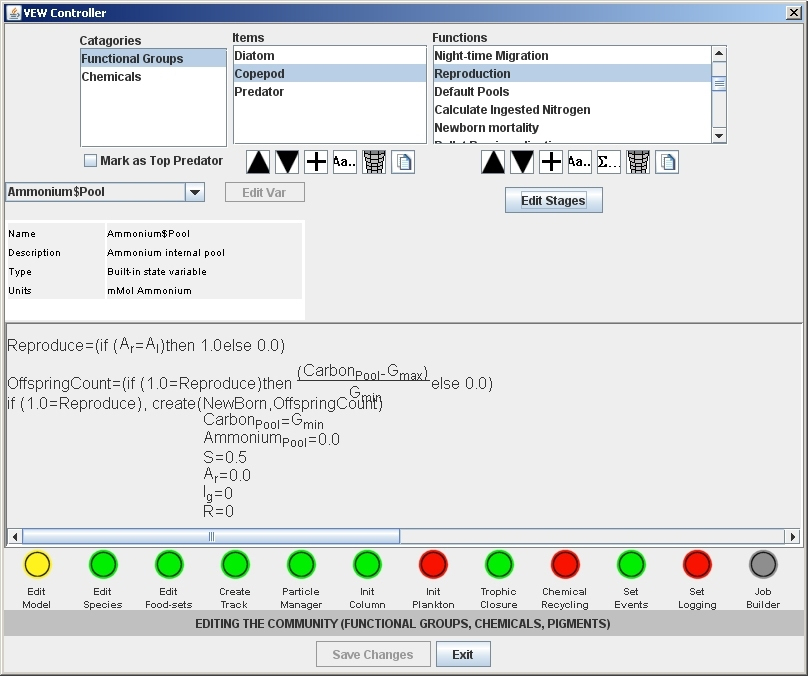
\includegraphics[width=0.7\textwidth,natwidth=808,natheight=676]{images/vew2007-10.jpg}
    \caption{Look at Virtual Ecology Workbench GUI of equation editor}
    \label{fig:VEW}
  \end{center}
\end{figure}

Virtual Ecology Workbench enables users to create simulation using
phenotypic equations in form familiar to them. It automatically
generates necessary code to represent environment and species
specified by user. The Lagrangian Ensemble metamodel
provides good trade-off of computational complexity and accuracy.
The metamodel computes emergent properties, the demography
of species population and biofeedback between agents and environment.
The simulation describes life history of every individual plankter
in the ecosystem to make it possible. Each agent in the simulation
behaves like a population of multiple identical plankters. Each
plankter in the ecosystem is contained in one of those agents.
Simulation created by VEW employ splitting and merging techniques
to ensure that that population is adequately represented and
that sampling is accurate where each agent can be subdivided into
multiple or two agents can be merged together. Therefore the
total number of agents can always stay within boundaries
defined by the user.

\subsection{Environment}\label{para:1d-phys}
\begin{figure}[H]
  \begin{center}
    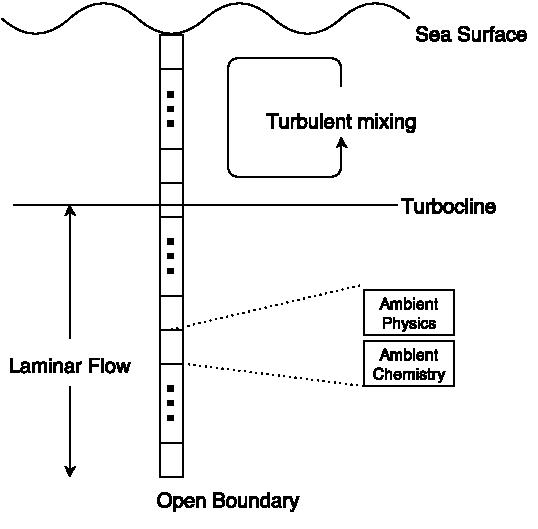
\includegraphics[width=0.6\textwidth,natwidth=473,natheight=466]{images/env-diagram.pdf}
    \caption{Physical environment in which VEW carries out the simulation}
    \label{fig:env}
  \end{center}
\end{figure}

Figure \ref{fig:env} illustrates the environment that is employed by VEW
to carry out its simulation. The physical environment as defined by \cite{Woods2005}
is a one-dimensional water column for us in open ocean where water depth exceeds 1km.
The vertical axis extends from the sea surface to depth of, typically, 0.5km.
VEW allows for the column to drift with ocean currents or be hoisted in place.
Solar and infra-red radiation, sensible and latent heat, water vapour
and other gases pass through the upper boundary while the lower is open
and allows detritus to sink through to the deeper parts of the ocean.
The physical model makes an assumption that even though the
water can flow freely through side walls of the environment it produces
zero flux divergence in every ecosystem property at all depths.

There are two reasons why approximation through one-dimensional model is
acceptable and will produce good results. First of all, the plankton being
modeled lives mostly in seasonal boundary layer of the ocean which has structure
controlled mostly by vertical fluxes. Secondly, the horizontal correlation
scale of the environment variables is typically two orders of magnitude greater
than the vertical scale. Planktons cannot usefully change their ambient environment
by swimming horizontally. However, many species of plankton do change their
ambient environment by swimming horizontally. This one-dimensional model is a very
good first approximation. It has to be noted though that the principal source
of errors arises from the neglect of mesoscale turbulence which is mostly correlated
in horizontal scale. Simulation of plankton ecosystems with mesoscale turbulence
requires three dimensional version of LE metamodel. In work by \cite{FluidityVEW}
the author shows how to integrate VEW generated models into general computational
fluid dynamics framework and demonstrates that the resulting system adjusts to
similar attractors as one-dimensional version.

\subsection{Functional Groups}\label{subsec:fg}

At the core of Lagrangian Ensemble modeling there are functional groups (FG).
Functional groups are the highest level grouping in marine biodiversity
parameter space. It defines set of variables that represent agent's internal
biochemical state. Furthermore it is used to define the set of phenotypic
equations that govern physiology and behaviour which are used to advance
agent to next time step.

\begin{figure}[H]
  \centering
  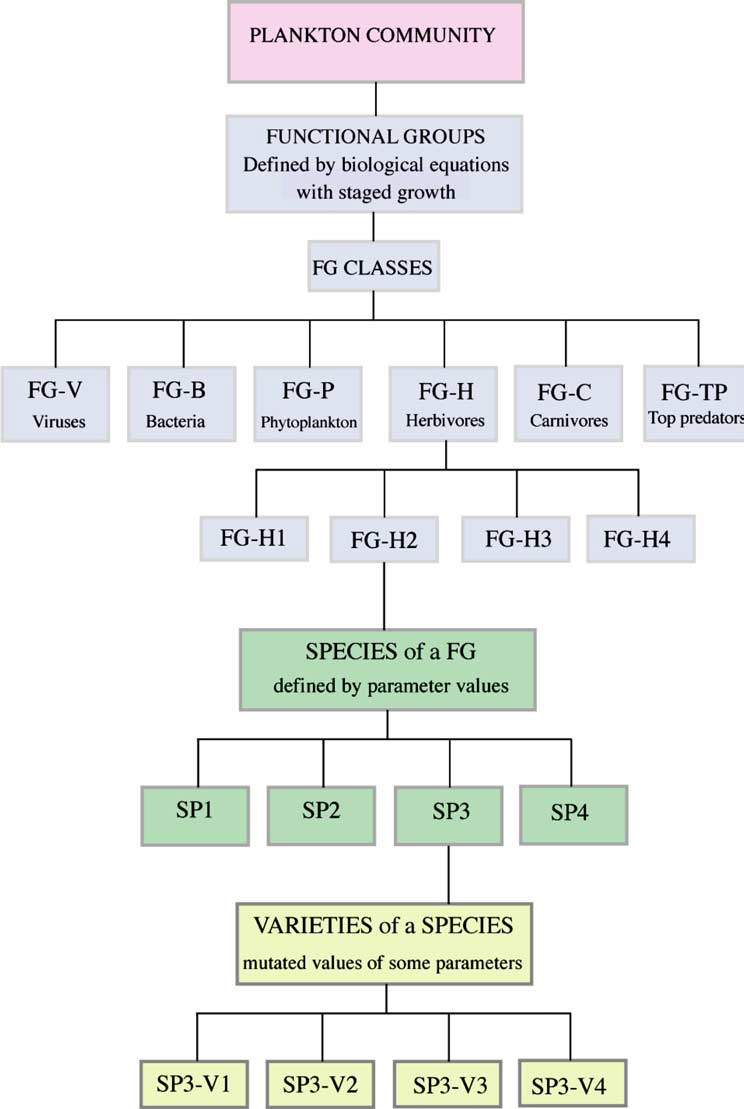
\includegraphics[width=0.7\textwidth,natwidth=744,natheight=1109]{images/fg.jpg}
  \caption{Plankton community according to \cite{Woods2005}
    with functional groups, species and varieties}
  \label{fig:fg}
\end{figure}

Figure \ref{fig:fg} shows grouping hierarchy of ecosystem modeling
objects. The plankton community in simulation consists of multiple functional
groups. Each of communities may be later subdivided into species. In case of
LE modeling species define parameter set for enclosing functional group set of
equations. Through parameter mutation we can achieve multiple varieties of
species. Going further down each species can be subdivided into traits.
Traits allow to factor in ecological adaptation in resource competition models.
As such traits are a way to incorporate evolution into ecosystem models
which is a current trend in modeling \cite{Clark20113823}.

The major difference in Lagrangian Ensemble model as proposed by
\cite{Woods2005} is the ability to capture life-cycle of an individual. This
feature is impossible to emulate in population-based approaches. As a
consequence each agent can have particular stage associated with it. Agent's
stage defines physiological processes currently active in subpopulation hence,
the phenotypic equations that are being used at particular timestep. The LE
allows for incorporation of growth, dormant stages and over-wintering as
seen in nature. The metamodel acknowledges the fact that physiological
behaviours of individuals may change over time and thus should be represented
in the model. Different growth stages constitute important source of intra-population
variability in ecosystem modeling.

\subsection{Model Specification - Planktonica}\label{subsec:planktonica}
The way in which model is specified in Virtual Ecology Workbench is through
Planktonica \cite{Planktonica}. Planktonica is a modelling language for
designing plankton. Arbitrary chemicals, with different action spectra to
represent pigmentation, can be used. Planktonica allows for encapsulation of
metamodel which describes basic rules in which simulation is carried out
like the definition of particle, the way the may interact and definition
of environment.

Planktonica creates the simulation code from the high level description
provided by the user. Thus it does not require programming knowledge.
The descriptions provided are transformed to an XML model which is
further enriched by later stages of VEW pipeline. Finally Planktonica
itself generates the code required to run the simulation for specified
model. Figure~\ref{fig:planktonica} Illustrates how the parts of the system
communicate together.

\begin{figure}[H]
  \centering
  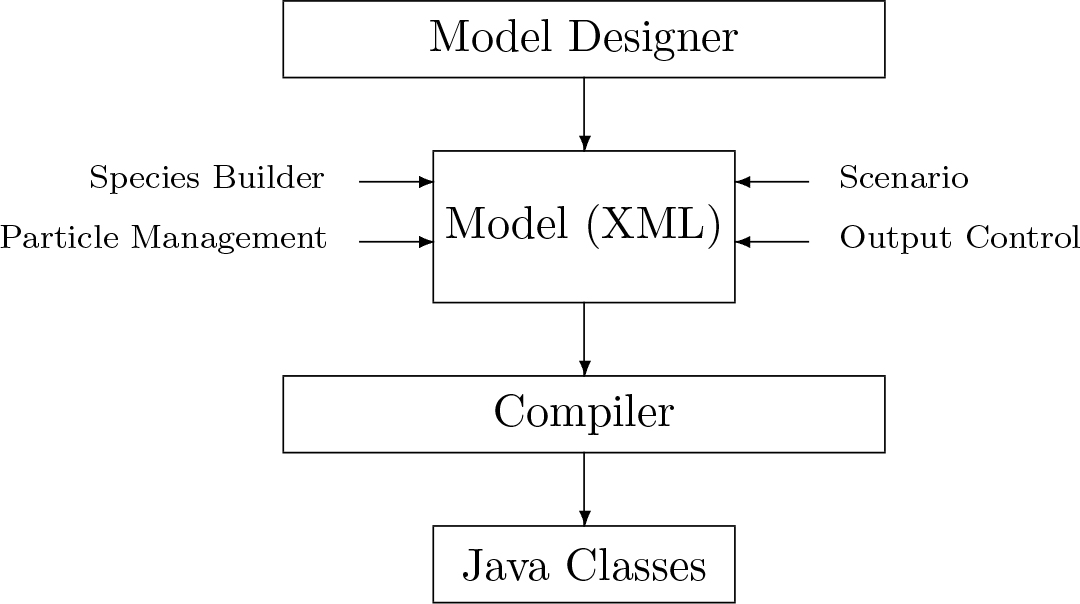
\includegraphics[width=0.7\textwidth,natwidth=1080,natheight=604]{images/planktonica.jpg}
  \caption{Schematic working of Planktonica taken from \cite{Planktonica}}
  \label{fig:planktonica}
\end{figure}

\subsection{Agents}\label{subsec:agents}
Lagrangian Ensemble metamodel has the ability to represent
multiple organism from same subpopulation into one agent.
Therefore plankton in the simulation can be described in
terms of primitive biological equations which are
observable in laboratory experiments. Instead of defining
each elements behaviour separately the LE metamodel uses
functional groups, species and stages to define set of
variables that govern its state and transitions.
Due to independence of agent updates from state all of the
biochemical processes can be defined once for any species
in particular stage. This is to the contrary to field models
where each property changes differently depending on a location
on a fixed mesh \cite{Woods200543}. Furthermore agents are able to
nondeterministically change their internal biological
state via stage transitions. In order to manage
those extra care has to be taken in particle management.

\subsection{Physics - Particle Management}\label{subsec:physics}
Due to individual based nature agent based model require a sampling
strategy to represent large number of plankters per cubic metre in the
ocean while keeping the problem computational feasible. This is achieved
in Lagrangian Ensemble metamodel via number-based up-scaling mechanism,
i.e. single agent represents multiple identical individuals. In order
to be able to compute demography of the population realistically
every individual has to occur in one of the agents present in the
environment. Due to the fact that number of individuals may change
significantly during particular time step. Therefore agent accounting
method is necessary to keep the number of agents during simulation
in desired range.

Restriction on number of agents are enforced by Particle Management.
The manager provides the trade-off between accuracy and speed of the
simulation. In order to enforce bounds specified by the user
the agent population is re-sampled using a continuous split/combine
algorithm. The number of agents is increased in a given region
by splitting the largest of agents in the set evenly until
the minimum threshold value is surpassed. Converse happens when
merging. The smallest agent in region are merged in pairs of two
and resulting agent has the weighted average of variables from source
set.

\begin{figure}[H]
  \begin{center}
    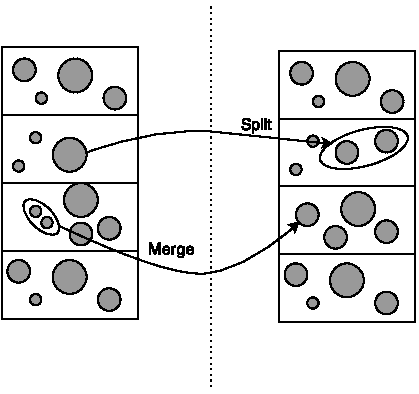
\includegraphics[width=0.4\textwidth,natwidth=366,natheight=342]{images/Split_merge.pdf}
    \caption{Example of Split/Merge in action}
    \label{fig:split-merge}
  \end{center}
\end{figure}

This method is illustrated in Figure \ref{fig:split-merge},
where a target density of four agents per level is requested.

\section{Fluidity}\label{sec:fluidity}
The biggest disadvantage of models generated by VEW is the 1D environment.
It does not allow for horizontal movement and according to authors
``serves as a good first approximation'' \cite{Woods2005}. It is still an approximation.

In work done by \cite{FluidityVEW} Fluidity, general-purpose
computational fluid dynamics software, has been adapted to incorporate
ocean modelling. Fluidity \cite{Piggot2008,fluidity} is capable of
solving Navier-Stokes equations and accompanying field equations on
arbitrary unstructured finite element meshes. The computation is
parallelised using MPI and uses adaptive remeshing to optimize the
underlying mesh structure at runtime. Therefore achieving computational
efficiency and focus on regions of interests. The resulting Fluidity-ICOM
provides ocean model capable of sub-grid scale parametrization to model
turbulent mixing as well as embedding of plankton biochemistry.

Fluidity is highly configurable via graphical user interface tool Diamond
which comprises larger scheme-driven description library Spud \cite{ham2009spud}.
Using the tool users are able to define properties to be computed during the simulation.
Fluidity has three types of fields \cite{fluidity}:

\begin{itemize}
  \item Prognostic fields are computed through solving partial different equations.
    User can specify discretisation used during solve phase as well as initial and boundary
    conditions via Diamond.
  \item Diagnostic fields are computed from other fields without solving a
    partial differential equation.
  \item Prescribed fields are defined by external sources. They can encapsulate a constant
    or a user defined function which can, i.e. be used to derive environment condition
\end{itemize}

\subsection{3D Particle Management}\label{subsec:3d-pm}
The key motivation for using Fluidity to model the physical environment
is the ability to introduce individual based plankton simulations in three
dimensional setting. With 3D meshes the impact of mesoscale turbulence,
only possible with turbulent ocean dynamics, on plankton simulations
can be investigated. In order to ensure correctness of the simulation
the interplay between ocean dynamics and ecological factors of marine
plankton ecosystem the ocean model has to be capable of resolving
turbulent flows at varying scales and resolutions.

VEW based models do not resolve turbulent nutrient dissipation within
surface mixed layer but enforces it. Fluidity has inherently different
model where it solves advection-diffusion equation with numerical eddy
diffusivity to achieve turbulent nutrient dissipation.
VEW generated simulation rely heavily on accurate convection based
cycle of mixed layer deepening. The key challenge is to integrate
mixed layer depth model used in VEW and Fluidity's advection-diffusion
equations. In order to achieve the desired effect K-profile parametrisation
is used alongside VEW's MLD model.

\myparagraph{Adaptive Remeshing}\label{para:remesh}
What makes Fluidity attractive for large scale simulations is its ability
to dynamically adapt the underlying mesh at runtime. The process minimises
discretisation errors and focuses resolution on regions of particular interest.
The adaptive mesh refinement uses anisotropic metric tensor field which
describes desired geometric properties necessary to minimise interpolation error.
The metric tensor can be formed from multiple fields and is computed using
Hessian of the fields under consideration. Therefore Fluidity's adaptive
mesh will have higher resolution in areas of steep gradients and coarser
in regions with smooth transitions.
From point of view of ocean modelling the ratio between horizontal
and vertical dimensions should be high. Particularly is mesoscale processes
are to be resolved. Fluidity has the ability to decouple vertical
and horizontal adaptation steps resulting in columnar mesh where elements
are aligned vertically and extruded from underlying horizontal two-dimensional mesh.
The vertical resolution is adapted independently of horizontal and allows
for linking between all columns to form a layered mesh.

\subsection{Model Specification - Python}\label{subsec:model-spec-py}

\begin{figure}[H]
  \begin{center}
    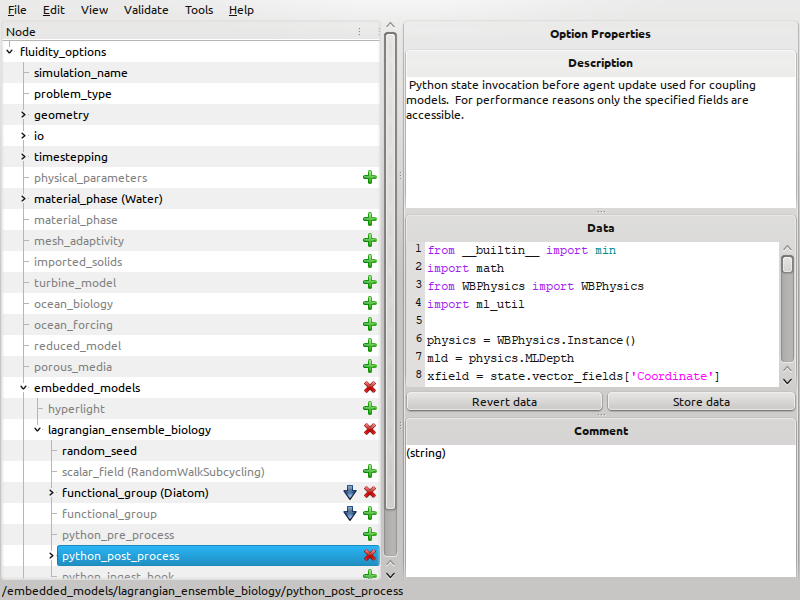
\includegraphics[width=0.7\textwidth,natwidth=800,natheight=600]{images/diamond.png}
    \caption{Diamond - Fluidity's configuration creator}
    \label{fig:diamond}
  \end{center}
\end{figure}

Python is used throughout Fluidity-ICOM implementation to provide flexible
interface which serves as a further customisation to configuration options.
The provided Python code is used to prescribe and manipulate field data.
Fluidity employs CPython via it's C-API to allow on the fly computation
of user provided options.

Diamond, show in Figure \ref{fig:diamond} is used in Fluidity to provide easy way to modify large
configuration files. Python code can be conveniently embedded via its
interface.

The embedded interpreter is used two fold
\begin{itemize}
  \item Space and time-varying field data - Space and time-varying field
data may be entered as a Python function to define prescribed fields
or enter the initial condition of a prognostic field.
  \item Internal State - Fluidity provides access to internal state
  and field data via Python interface. Through this interface
  the user can define own diagnostic algorithms where diagnostic
  field values are set by user defined Python functions. The interface
  may also be used to define ecology models by specifying relevant
  source and absorption terms of the prognostic fields representing
  the ecosystem elements.
\end{itemize}

\section{LERM}\label{sec:lerm}
Throughout this thesis the model employed is based on
Lagrangian Ensemble Recruitment Model (LERM) as first designed
by \cite{FisheriesRecruitment}. LERM is a
fisheries recruitment model that uses four trophic levels to
model the effects of predation and competition on squid recruitment.

\subsection{Simple LERM}\label{subsec:lerm-simp}
While the original model provides realistic example in order
to focus on performance aspects of simulation as simplified version
is used. Thus only Diatoms, plant-based plankters, are present
as agents. Top level predators as well as Copepods (animal-based plankton)
are ignored in this version of the model. There is no predation
between agents, hence there is no need to simulate ingestion.
While those restrictions focus biological environment we will also
disregard bio-optical feedback and read physical environment
information: temperature, visible irradiance, level of turbocline
layer and depth of water column, from files generated by
full Java based VEW simulation. The simulation is run for 2 years
with time step resolution of 30 minutes. Therefore we can observer
yearly cycles which we can use to determine simulation's correctness
when modified. The 30 minute time step resolution is a simplification
which allows to avoid agent movement since effectively due to ocean
currents and turbulence the new location can be random in turbocline
region.

\subsection{Simple LERM in Fluidity}\label{subsec:lerm-simp-fluid}
The Simple model just explained has sever limitations when it comes
to environment and particle management. Furthermore it's based on
on VEW model instead of Fluidity one. Due to complexity of environment
and ability to model arbitrarily complex systems simple fluidity
LERM has to take into account spatial layout of agents. However,
those are handled by Fluidity itself and we only need to provide
configuration options. Agent update code for Fluidity based simple
LERM model is almost identical to VEW based model. Only changes
necessary are due to Fluidity-ICOM having proper Python API (outlined
in \cite{FluidityVEW}). Therefore stage constants, agent dropout (siking)
and agent growth effects had to be replaced by function calls.


\section{Parallelisation}\label{sec:para}

\subsection{OpenMPI}\label{subsec:openmpi}
Message Passing Interface is a way of distributing computation
amongst several machines via network connection. Each of the
machines (nodes) in the system is able to issue and receive
messages which are a way to synchronize and distribute data.
OpenMPI \cite{gabriel04:_open_mpi} is a result of merger of several MPI libraries, like
LAM/MPI, LA-MPI, and FT-MPI. It aims to standardise the implementation
and improve interoperability. Thus reducing the burden on
end users and increasing adoption. It provides production-quality
MPI-2 implementation. Currently OpenMPI is de-facto the MPI
library. Apart from being a quality MPI implementation is to
facilitate third-party research and creation of independent
add-ons.

\subsection{OpenMP}\label{subsec:openmp}
While OpenMPI focuses on distributing workload amongst different
machines OpenMP \cite{OpenMP4.0} is used to distribute tasks in one machine amongst
several cores. Due to it's memory oriented nature there's a significant
penalty incurred when operating across different cache domains.
OpenMP aims to provide compiler directives, library routines, and environment variables
for shared-memory parallelism in C, C++ and Fortran programs.

In contrast to other multithreading approaches OpenMP provides high
abstraction level thus enabling portability. The portability of OpenMP directives
is ensured by runtime library which is platform dependent part of implementation.
The directives it introduces focus on single program multiple data
(SPMD) constructs, tasks, worksharing and synchronisation.
Furthermore the library provides means of sharing and privatizing
data across threads.

OpenMP only covers user-directed parallelization, where programmer explicitly
states actions which are to be taken by compiler to make program parallel at runtime
Any implementation is not required to check for data dependencies, data conflicts,
race conditions, or deadlocks which may occur in multithread programs.
The specification does not cover compiler-generated automatic parallelization and
directives to the compiler to assist such parallelization.

Since OpenMP is tightly integrated with the compiler it is non-trivial to
understand types of transformation that are performed to make program parallel.
Listing \ref{list:openmp-dir} and \ref{list:openmp-run} shows one of the transformation that is performed.

\begin{lstlisting}[
  caption=Code with OpenMP directives,
  label=list:openmp-dir,
  language=c
]
#include <omp.h>
void main() {
  #pragma omp parallel
  {
    int ID = omp_get_thread_num();
    printf(“Hello world(%d)”, ID);
  }
}
\end{lstlisting}

\begin{lstlisting}[
  caption=Code from \ref{list:openmp-dir} with substituted runtime library calls,
  label=list:openmp-run,
  language=c
]
void __ompregion_main1(...) {
  int ID = ompc_get_thread_num();
  printf(“Hello world(%d)”,ID);
} /* end of ompregion_main1*/

void main() {
  ...
  __ompc_fork(&__ompregion_main1,...);
  ...
}
\end{lstlisting}

\subsection{Isoefficiency}\label{subsec:isoeff}
Isoefficiency is a measure of how in relation to growth in number of parallel execution units the working set has to grow in order to maintain same efficiency of the system. In general with growing working set size given constant number of processors the efficiency increases while the inverse happens when working set size is constant and number of parallel execution units increases.
\begin{equation}\label{eq:isoeff} W = \dfrac{E}{1-E}T_o(W,p) \end{equation}
\ref{eq:isoeff} describes relation between working set size and efficiency for parallel system as defined in \cite{grama2003introduction}.
For any scalable system efficiency can be maintained at a fixed value if the ratio \[\dfrac{T_o}{W}\] is kept at a constant value.
Let \[K = \dfrac{E}{1-E}\] be a constant depending on the efficiency to be maintained. The we have
\begin{equation}\label{eq:isoconst} W = KT_o(W,p) \end{equation} Knowing properties for a particular system we can obtain value of W
as a function of p which dictates the rate at which working set size has to grow in order to maintain fixed efficiency.

\subsection{Python Multithreading}\label{subsec:mult-py}
Python as a programming language dates back to beginning of 90s. Since that
time it has grown to be one of the most widely used general purpose scripting
languages. Due to its high abstraction level it allows expressing concepts in
few lines of code. Furthermore it provides large standard library.

Python is a truly multithreaded language. Each of the threads that are spawned
by interpreter are first class operating system threads. As such Python gives
ability to write applications running on large machines. There's a caveat, namely
the Global Interpreter Lock (GIL). Due to GIL besides threading concurrency model
Python provides process level concurrency. Since each process has its own address
space and memory they do not interfere with each other and can run in parallel.
Due to inter process communication there is a significant overhead incurred
when passing values around between processes. In order to mitigate the drawbacks
of memory passing Python aims to provide non blocking interfaces for I/O and
networking operations which effectively make explicit threading redundant. However,
Python does not have a good solution for threading CPU intensive programs. There are
numerous extensions, most prominent of which are NumPy and SciPy. Those libraries aim to provide
true parallelism for CPU intensive operations. However, they achieve this effect
not in pure Python but by delegating the computation to external C or Fortran modules
which can run unaffected by GIL.

It has to be noted that Python as a language has multiple implementations. Most
widely used are CPython (reference implementation), PyPy (CPython compatible implementation
with JIT capabilities), IronPython (Python implementation in C\#)
and Jython (JVM based implementation). The GIL problem only applies to CPython
and implementations that are compatible with it. Given the fact that other
versions don't have widespread adoption Python is often exclusively associated
with CPython. Given the fact that majority of Python modules are written to conform with
CPython API any implementation without CPython compatibility stands little chance
of widespread adoption and success.

\subsection{Global Interpreter Lock (GIL)}\label{subsec:GIL}
The Python reference implementation (CPython) has been written with Global
Interpreter Lock. What GIL does is to ensure that only one thread at a time
modifies the internal memory of interpreter. This in turn is necessary
due to CPython memory model. By using reference counting for garbage collection
CPython removes burden of explicit memory management, however, for the
scheme to work the reference counts have to be accurate. Therefore whenever
an object in Python is created and modified the thread has to acquire an
exclusive lock for memory modification. As a result of GIL regardless
of number of threads if the application wants to interpret Python code
it will use only one thread. This behaviour is a bottleneck for CPU
intensive applications rendering them exclusively single threaded.

\myparagraph{Removing GIL}\label{para:remove-gil}
With shift from faster processors to more cores per processor in CPU
design the GIL had become a central issue to threading Python code.
First proposal to remove GIL from Python occurred in 1999 when Greg Stein
replaced GIL in Python 1.5 with fine-grained locks \cite{Guido:GIL}. However, the resulting
code was almost two times slower than version with global lock,
moreover there was no clear gain from threading the interpreter due
to lock contention being a bottleneck. As a result the changes have
disappeared over time. The need to remove GIL lessened over time
with development of modules which operate in pure C or Fortran code
and therefore can be treaded. In case of I/O and networking the
problem is mitigated with asynchronous calls. GIL remains issue
only for CPU intensive tasks.

There are downsides to removing GIL though. Without guarantees from
the interpreter that extension will can be executing only once at
a time the development of them become more difficult. Without GIL
developers of 3rd party modules has to make their code thread-safe
which can prove to be difficult and require significant effort.

\section{Embedding Python in C}\label{sec:python-embedding}
As a result of CPython being written in C it exposes native C API for
programs that wish to use its facilities. Thus Python code can be
interpreted without explicitly invoking interpreter in another process.

\subsection{Python/C API}\label{subsec:python-capi}
The listing \ref{list:python-embed} illustrates the calls necessary
to execute Python code from C program. The example only shows
high level embedding where Python is still responsible for parsing
code and there is no interaction between application and interpreter
state.

\begin{lstlisting}[
  caption=Embedding Python code (taken from Python documentation),
  label=list:python-embed,
  language=c
]
#include <Python.h>

int main(int argc, char *argv[]) {
  Py_SetProgramName(argv[0]);  /* optional but recommended */
  Py_Initialize();
  PyRun_SimpleString("from time import time,ctime\n"
                     "print 'Today is',ctime(time())\n");
  Py_Finalize();
  return 0;
}
\end{lstlisting}

In order to achieve complex interaction we would have to dig
through API reference to understand how Python represents variables
internally and find correct ways to modify them. Needless to say
despite very thorough documentation, writing C instead of Python
greatly increases verbosity of the program. Owing to the fact
that Python has a stable API better approaches have been proposed,
most significant of which is Cython. Cython allows users to write
Python like syntax which in turn is compiled to Python C/API
with appropriate function calls and boilerplate generated
automatically. Cython gives the flexbility of Python while allowing
compatibility with C applications without the need to understand
inner workings of CPython.

\subsection{Cython}\label{subsec:cython}
Cython \cite{Cython} is an optimising compiler which extends Python syntax in order
to allow mixed compilation to Python C/API and direct C/C++. Cython
relies on principle that knowing size and contents of the variable,
namely the type, allows the compiler to generate efficient machine
code to represent the operation. Without types and type inference
mechanisms the interpreter has to assume nothing and execute code
that can handle all cases, more efficient code can almost always
be generated. Cython extends Python syntax to allow for defining
C/C++ like elements. As such it provides facility for declaring types
of variables. Furthermore it allows for easy wrapping of C/C++ code
thus enabling seamless integration.

Listing \ref{list:python-cython} shows sample Cython code with all possible
annotations. While such code can be more concisely expressed in Python, the type
annotations can give significant speed improvements. The Cython version is
\emph{16 times} faster than pure Python version of this function (shown in Listing
\ref{list:python-annot}).

\begin{lstlisting}[
  caption=Sample Cython code,
  label=list:python-cython,
  language=python
]
cpdef int sumTo(int num):
    cdef int c = 0
    cdef int i
    for i in range(num + 1):
        c = c + i
    return c
\end{lstlisting}

\subsection{Code annotations}\label{subsec:cython-code-annot}
As a consequence of providing type annotations it is possible to generate
pure C/C++ from Cython code. The generated code will not rely on Python/C API
while preserving compatibility with Python and allowing to fall back to it if necessary.
Cython provides annotation facility to easily associate source code with
corresponding generated code. Through line colouring it is easy to asses how
expensive, in terms of lines of code, given line of Cython code is.

\begin{lstlisting}[
  caption=Python code annotated by cython,
  label=list:python-annot,
  language=python,
  linebackgroundcolor={
    \ifnumequal{\value{lstnumber}}{1}{\color{cython-line-1}}{}
    \ifnumequal{\value{lstnumber}}{2}{\color{cython-line-2}}{}
    \ifnumequal{\value{lstnumber}}{3}{\color{cython-line-3}}{}
    \ifnumequal{\value{lstnumber}}{4}{\color{cython-line-4}}{}
    \ifnumequal{\value{lstnumber}}{5}{\color{cython-line-5}}{}
}]
def sumTo(num):
    c = 0
    for i in range(num + 1):
        c = c + i
    return c
\end{lstlisting}

Listing \ref{list:python-annot} shows output produced by cython annotate
for pure python version of the code from Listing \ref{list:python-cython}
The more saturated yellow on the line is the more lines it will take in
the generated C code. If the line is white the source code line will have
direct translation to one line of C/C++ code. If all of the code translates
directly then it isn't touching any of Python internals and we effectively
have eliminated Python as a runtime requirement. Listing \ref{list:python-cython}
is an example of code that will translate directly to C.

\subsection{Python embedding with Cython}\label{sec:embed-cython}

Main objective of Cython project is to facilitate embedding C/C++ code in
Python programs. It can provide bindings in opposite direction allowing
to call \lstinline{cdef} functions from C code. While it isn't possible
to directly invoke Python function it is possible to write a wrapper
that will be accessible from C which in turn will have Python function
available to it. For instance Listing \ref{list:cython-public-module}
shows two functions which are declared as \lstinline{public} which means
that a C header file will be generated upon compilation. If the code
resides in a modulename.pyx file a modulename.h will be generated containing
prototypes for all public functions.

\begin{lstlisting}[
  caption=Cython public function definitions,
  label=list:cython-public-module,
  language=python
]
cdef public void _updateLivingDiatom(float * vars, float * rel, float temp, float vis_irradiance, float * chem) nogil:
cdef public void _updateDeadDiatom(float * vars, float * rel, float temp) nogil:
\end{lstlisting}

Then from C code we can include the Cython module and access all public methods as
shown on Listing \ref{list:c-cython-public-usage}.

\begin{lstlisting}[
  caption=C code showing usage of Cython public interface,
  label=list:c-cython-public-usage,
  language=c
]
#include <Python.h>
#include "modulename.h"

void cython_call() {
    Py_Initialize();
    initmodulename();
    ... call _updateDeadDiatom or _updateLivingDiatom
    Py_Finalize();
}\end{lstlisting}

It is crucial to call \lstinline{initmodulename()} since it serves as a setup
function for the module, it executes any global code (outside of any function)
and initializes Python environment. Calling functions from module is still
possible given theydon't rely on any of those. We will exploit this fact in
when implementing Python compilation in Fluidity.

\chapter{Simple LERM Model}\label{ch:opt-simpl-lerm}
In work done by \cite{FluidityVEW} it has been shown that Langrangian
Ensemble metamodel can be successfully embedded in unstructured
three-dimensional mesh. The work mentions that resulting software while
flexible has severe performance limitations. The core Fluidity code
is heavily optimized and relies on OpenMPI and OpenMP to distribute
the work to available machines. However, due to flexibility of model
specification through Python and the limitations of Python outlined
earlier (GIL) the biological aspect of the simulation is effectively
single threaded. There is no need for the update loop of the simulation
to be run sequentially. Since all of the agents are independent
entities and any interaction are resolved only after the update had
taken place they can be updated in parallel.

The original Virtual Ecology Workbench does not exhibit this problem.
By using domain specific language for defining the agents behaviour
it can use code generation techniques to produce optimal and threadable
code. Furthermore by using Java it does not exhibit issues with GIL
as Python does. JVM is an extensively tested and developed for architecture
and its performance is close to native code while providing easy to use
threading model.

The aim of this work is to investigate what performance gains can be
achieved if the bottleneck due to Python GIL can be overcome while
preserving the flexibility that original version offers. The original
from Fluidity-ICOM relies on Python C/API to provide the update code
with internal state values.

Previously we have seen that Cython offers greater degree of flexibility,
than directly targeting the API, and possibility of generating GIL free
code. Therefore by using Cython we will try to provide cleaner implementation
and avoid the performance bottleneck.

Fluidity-ICOM is a complicated piece of software and provides a lot more
functionality than necessary for the outlined investigation to be carried
out. By considering Simple LERM model with embedded Python code for agent
agent we achieve minimal example that exhibits same characteristics. Later
we will see how the solution implemented in Simple LERM model can be ported
to Fluidity-ICOM. The difference in implementations comes from the fact
that Fluidity-ICOM has enable runtime configuration and as such the code
that has to be optimised is only known at runtime.

\section{Experimental setup}\label{sec:exp-setup}

Benchmarks and profiler output presented in this work had been carried
on three different machines. Bulk of benchmarks have been carried
out on a machine with quad core Haswell CPU (i7 4770 @ 3.4 GHz) with
16 GB of RAM (memory capacity is not a problem for simulation in
question, memory latency on the other hand is). Care
had been taken to ensure that hyper threading does not distort the results.
To tests scalability and multi threaded behaviour of the simulation further
additional tests had been run on machine with 4 Sandy Bridge CPUs
(8 cores each - E5-4650 @ 2.7 Ghz) with 500 GB of ram. However, only 2 CPUs
have been used as the performance profile is not likely to change when
increasing number of CPUs further. For each of the versions of code and
number of threads 5 runs have been carried out to remove some of the noise.

Throughout the testing the simulation has been compiled using GCC 4.9.0
compiled from source on respective machines. All of the simulations have
been run with ``-O2'' optimisation flag. Cython compiles extension by
default at this optimisation level. Increasing optimisation level
(to ``-O3'' and ``-Ofast'') and specifying ``-march=native'' did not bring
any performance increase therefore was dropped from testing. To determine
appropriate flags for embedding Python \lstinline{python-config --includes}
have been used for includes and \lstinline{python-config --ldflags} for
link time library location resolution.

The profiler output, however, has been obtained with different compilation
flags and on different machine - quad core Haswell CPU (i7 4750 @ 2.0 GHz)
and 16 GB RAM. This is mostly due to VTune being a GUI program and a such it's
fastest to use it from machine with physical connection.
To allow profiler properly resolve all symbols at runtime, the simulation
was compiled with ``-Og'' (recommended optimisation level for debugging)
and ``-g''. Those two options can degrade performance significantly compared
to ``-O2''. Therefore profiler output should be treated only in relative
terms and as a guidance to where in program the performance is lost. The
simulation was profiled with 4000 agents to allow analysis of whole program
run. For slower code versions the execution time was a significant bottleneck
of benchmarking and profiling.

\section{Reference Implementation}\label{sec:ref-impl}

The simple model we will consider is a C implementation of simplified
LERM-PS model as described previously in \ref{subsec:lerm-simp}. In this
model we consider only development of Diatoms in fixed water column 500
meters deep. The physical environment is not simulated but read from
file which has been generated by full VEW simulation.

\begin{figure}[H]
  \begin{center}
    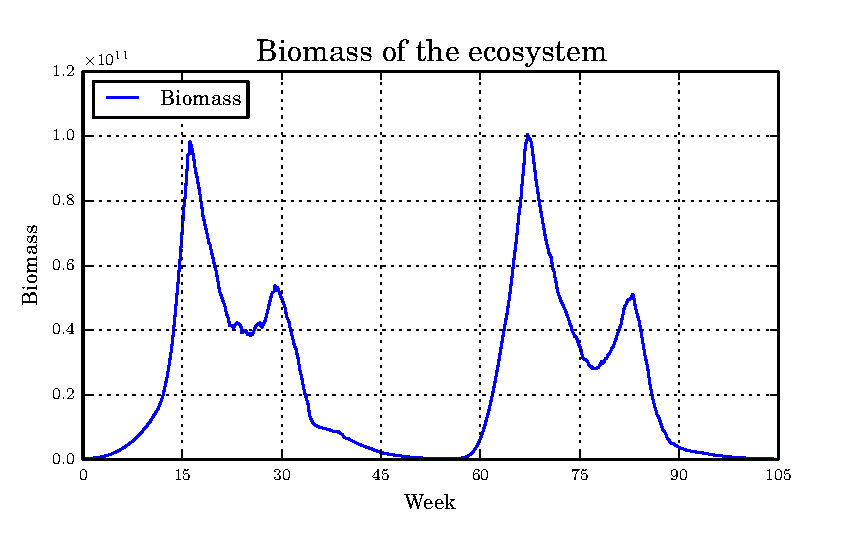
\includegraphics[width=\columnwidth]{graphs/master-bio.eps}
    \caption{Biomass of the ecosystem over time.}
    \label{fig:master-bio}
  \end{center}
\end{figure}

The simulation has a characteristic biomass curve, Figure \ref{fig:master-bio}.
VEW based simulation are stable therefore we can use the shape of it to
determine the correctness of our changes. There is clear bloom period at the
beginning of the year when the ecosystems biomass rises sharply.

\begin{figure}[H]
  \begin{center}
    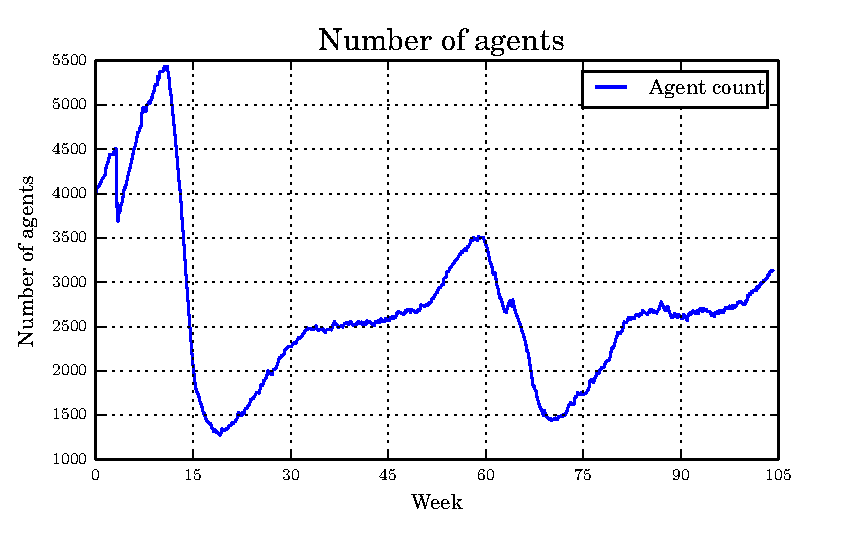
\includegraphics[width=\columnwidth]{graphs/master-ag.eps}
    \caption{Number of agents in simulation.}
    \label{fig:master-ag}
  \end{center}
\end{figure}

The agent count show in Figure \ref{fig:master-ag} is also characteristic
for the simulation. Due to seeded random number generation the shape of
the curve should be preserved. We can notice that agent count follows biomass
- larger biomass of the system the more the agents to  represent it.

The simulation itself is an update loop with logic for loading the
environment and storing results. As such it can be summarized by
Listing \ref{list:vew-main-loop}

\begin{lstlisting}[
    caption=Main loop of Simple LERM Model,
    label=list:vew-main-loop,
    language=c,
]
for (t = 0; t < 35040; t++) {
  readPhysics();
  mixChemistry();
  updateAgents();
  updateChemistry();
  particleManagement();
}
\end{lstlisting}

Since our target software has fundamentally different environment management
and initialisation, the attention is focused on \lstinline{updateAgents()}
function. That is the place where the embedded Python will get executed
and it contributes bulk of the execution time. Changes to other parts
of the code will be carried out only to allow reliable parallelisation
and correctness of results in multithreaded execution model.

Python is a significantly higher level language than C. Apart from making
the code threadable, the single thread performance should not be sacrificed.
Hence, we begin by benchmarking this implementation and will treat it as
our baseline for performance comparison.

\begin{figure}[H]
  \begin{center}
    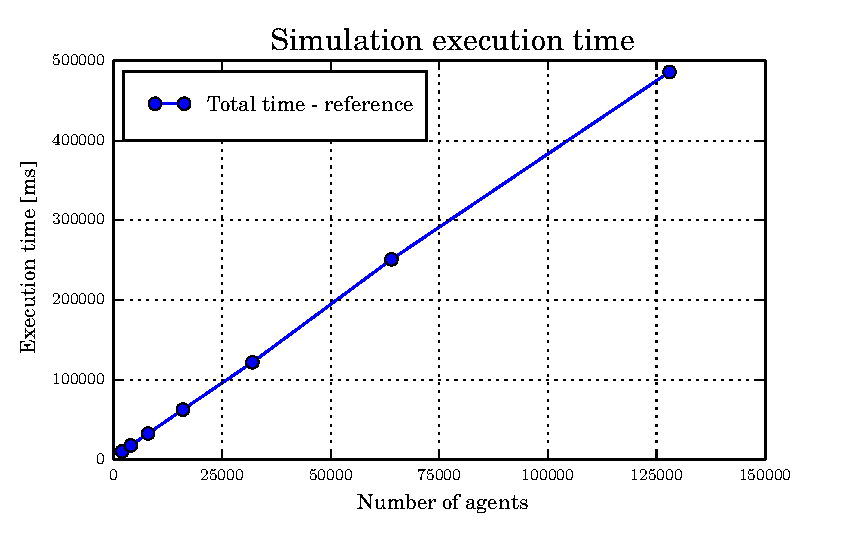
\includegraphics[width=\columnwidth]{graphs/master-perf.eps}
    \caption{Total execution time of simulation for reference version.}
    \label{fig:master-perf}
  \end{center}
\end{figure}

Table \ref{table:reference-timings} contains exact values used to plot the Figure
\ref{fig:master-perf} for reference. Furthermore breakdown between agent update,
particle management and environment is provided. We can see that the single threaded
version scales linearly in the presented range.

The VEW C based simulation has a lot of advantages from performance perspective.
There's no data abstraction thus all data is allocated in arrays. The memory
is over allocated to avoid slowdown due to \lstinline{malloc}. The data is
stored in plain arrays which guarantee continuous layout in memory. Furthermore
as the update code performs only arithmetic operations, the closer to hardware
we are the faster the operation, this is where C has an advantage over Python.
We shall see how we can mitigate penalties caused by higher level of abstraction,
it won't be possible with some restrictions though, which will be described later.

\begin{table}
  \begin{center}
    \begin{tabular}{|c||c||c|c|c|}
    \hline
    Number of agents & Total [ms] & Update [ms] & PM [ms] & Env [ms] \\ \hline
     2000            &  10367                    &  8949             &  201                     &  1117                        \\
    4000             &  17794                    &  16243            &  336                     &  1115                        \\
    8000             &  32749                    &  30901            &  630                     &  1118                        \\
    16000            &  62708                    &  60207            &  1279                    &  1120                        \\
    32000            &  121979                   &  118034           &  2720                    &  1122                        \\
    64000            &  251018                   &  242488           &  7230                    &  1180                        \\
    128000           &  486010                   &  467940           &  16822                   &  1139                        \\ \hline
    \end{tabular}
    \caption {Reference C version}
    \label{table:reference-timings}
  \end{center}
\end{table}

\begin{figure}[H]
  \begin{center}
    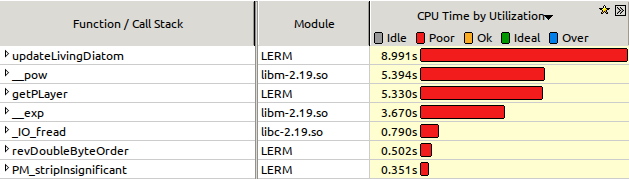
\includegraphics[width=0.7\textwidth,natwidth=629,natheight=179]{images/vtune-master.png}
    \caption{VTune output for simulation run of reference version}
    \label{fig:vtune-master-perf}
  \end{center}
\end{figure}

From VTune output in Figure \ref{fig:vtune-master-perf} we can see that this
version does not have any obvious bottlenecks. The simulation spends significant
amount of time in \lstinline{updateLivingDiatom}, \lstinline{__pow} and
\lstinline{__exp} functions which are pure arithmetic. The \lstinline{getPLayer}
is the possible performance gain for this version. This function finds corresponding
physical layer for agents location in the water column. It is called for all of the
\lstinline{updateLivingDiatom} calls to provide physical environment information.
However, as the Fluidity-ICOM is fundamentally different in this aspect and does
not have similar issues the code will be left as is. VTune will be used throughout
to guide the next steps and provide confirmation that given piece of code in
fact causes slowdown.

\section{Embedding Python}\label{sec:embed-py}
First step is to perform the embedding of Python. In order to do this the
we let Cython generate appropriate C functions and header file.
Then in turn those functions will include provided agent update code.
Hence, if the agent update code needs to be changed the simulation
code does not have to be recompiled (important requirement if porting
to Fluidity is to be useful). The necessary modifications to the simulation
do not require more than what is shown in \ref{sec:embed-cython}. What is left
is replacing the native C update functions with calls to Python versions
and propagating the return values as to preserve semantics of simulation.

The important part is the glue code that performs data transformation from
C to Python. As memory can be a significant bottleneck and constant copying
data back and forth will degrade performance rapidly care has to be taken
to ensure copy-free data passing. Furthermore since in Python the agent
variables are represented as dictionaries while in C they are simple arrays
a wrapping mechanism has to be provided to ensure consistent semantics of
code. Python represents everything as an object inside the interpreter.
As a result every operator actually calls certain function on object in
question. Fortunately CPython, as C++, allows for operator overloading,
therefore allowing us to create a wrapper for an array that behaves
like dictionary.

\begin{lstlisting}[
    caption=Python wrapper for agent array,
    label=list:array-adapter,
    language=python,
]
cdef object agentNames = {
    "AmmoniumIngested" : 0,
    ...
    "Stage"            : 12
}

cdef class AgentWrapper:

    cdef float * array

    cdef void setData(self, float* vars):
        self.array = vars

    def __getitem__(self, key):
        return self.array[agentNames[key]]

    def __setitem__(self, key, value):
        self.array[agentNames[key]] = value
\end{lstlisting}

\myparagraph{Cython cdef classes}\label{para:cython-cdef}
Beside supporting built-in Python classes Cython also provides second kind of
class: extension types, sometimes referred to as “cdef classes” due to the
keywords used for their declaration. They serve the purpose of mixing C and
Python semantics. Such classes are restricted compared to Python's due to
necessity of conforming to C standards. As a result they are more
memory efficient and faster than generic Python classes. The main difference
comes from the fact that they use C struct to store fields and methods instead
of Python dict. This enables them to store arbitrary C types without requiring
Python wrapper and accessing fields and methods directly at C level without
Python dictionary lookup. Generic Python classes can inherit from cdef classes
but converse is not possible. Since Cython requires to know the complete inheritance
hierarchy to properly lay out the C structs, and limits it to single inheritance.
Python classes, however, can inherit from any number of Python classes and
extension types both in Cython and pure Python code.
\\

\begin{figure}[H]
  \begin{center}
    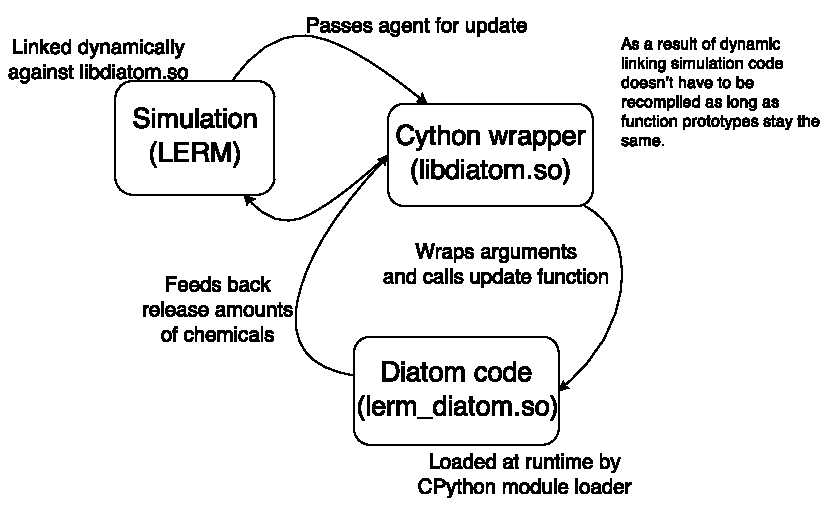
\includegraphics[width=0.7\textwidth,natwidth=731,natheight=441]{images/embed-diagram.pdf}
    \caption{Diagram illustrating high level code interactions and loading}
    \label{fig:embed-diagram}
  \end{center}
\end{figure}

Figure \ref{fig:embed-diagram} shows how the resulting code works to enable dynamic
code loading and ensure correctness of the result. In this version though the
agent code is not compiled to shared object by only loaded and interpreted by CPython.
This proves to be a significant performance hit which Figure \ref{fig:cython-perf} illustrates.
Bear in mind that the y axis has one order of magnitude larger values. On average the
naive embedding performed via Python C/API is \emph{35 times} slower than reference
C version. This is not a good sign if we want to achieve comparable performance even
with multiple threads.

\begin{figure}[H]
  \begin{center}
    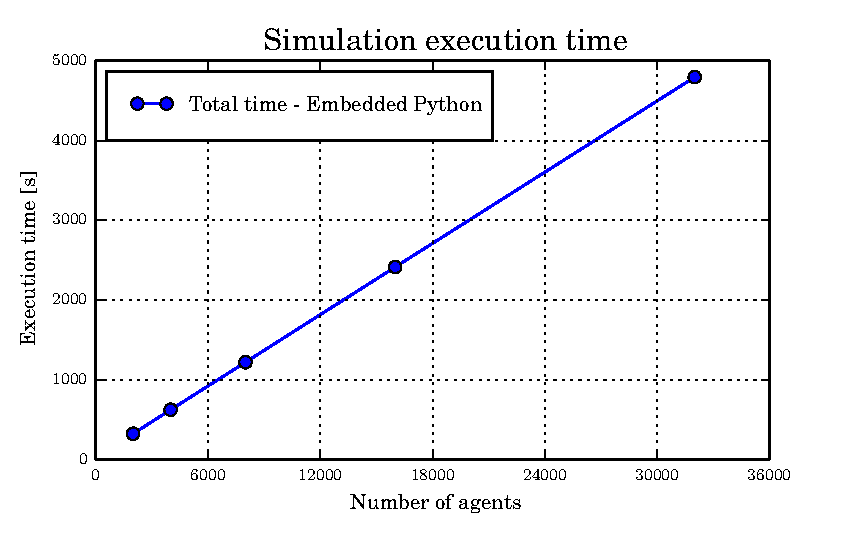
\includegraphics[width=\columnwidth]{graphs/cython-perf.eps}
    \caption{Total execution time of simulation for embedded python version.}
    \label{fig:cython-perf}
  \end{center}
\end{figure}

\subsection{Finding Bottlenecks}\label{subsec:python-embed-bottleneck}
From the Figure \ref{fig:cython-perf} we see a steep
degradation in performance that happened when the work had been delegated
to Python. Since the resulting code is still single threaded the GIL is
not an issue here. What is happening though is change in operation semantics
(Python doesn't have types, hence cannot generate optimised code for primitive types)
and memory accesses (array to dictionary).

To fully understand the extent to which those two factors impacted performance
VTune has been used for analysis.

\begin{figure}[H]
  \begin{center}
    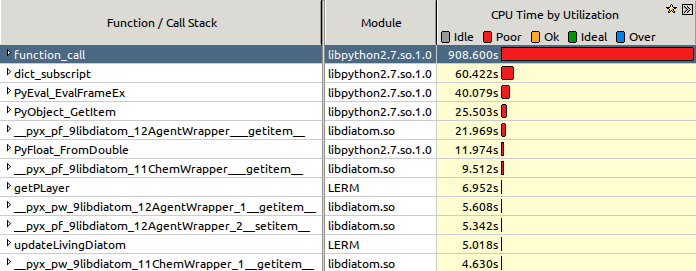
\includegraphics[width=0.7\textwidth,natwidth=696,natheight=271]{images/vtune-cython-pure.png}
    \caption{Vtune output for simulation run using Python update code}
    \label{fig:vtune-cython-perf}
  \end{center}
\end{figure}

From output of VTune shown in Figure \ref{fig:vtune-cython-perf} we see
that due to dynamic nature of Python we have limited insight into actual bottlenecks,
however, it is clear that the the agent update code should be investigated further.

Since the agent code is imported via \lstinline{import diatom} the whole of its body
is managed by Python interpreter (providing debug symbols for Python installation did
not help function name resolution). As a result any code that is directly imported via
Python mechanism is a black box from optimisation perspective. However, if we already
use Cython we can statically compile the agent update code as an extension
to be able to investigate parts of it further. That is where Cython helps
us further. Being targeted as easy way to create Python modules the changes necessary
are minimal - adding only another source file to distutils setup script.
Since we have to pass the update code through compiler to obtain meaningful profiler
output other optimisations can be introduced. We need any possible feature
in order to eliminate the performance penalty that has just been introduced.

\section{Typing update code}\label{sec:embed-py-type}
The difference Cython makes to Python is that it introduces typing in order to generate
efficient code. With agent update code being a pure Python implementation there is
potential for performance improvement without changing the function definitions
and the arguments passed. Section \ref{subsec:cython} shows that fully annotated
code can be significantly faster, however, there types are specified for every
variable present. We will limit the typing to just the code within the agent update.
This task is simplified by the fact that all of the computation inside the update
code are performed on floating point numbers. Hence, for any variable defined we
only have one choice for its type.

\begin{figure}[H]
  \begin{center}
    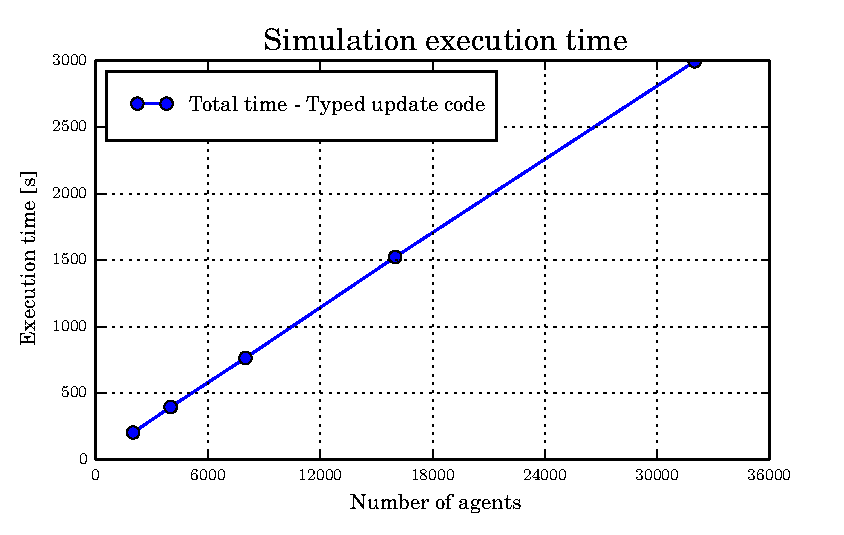
\includegraphics[width=\columnwidth]{graphs/cython-typed-perf.eps}
    \caption{Total execution time of simulation for embedded python version with type
    annotations for update code body.}
    \label{fig:cython-typed-perf}
  \end{center}
\end{figure}

Figure \ref{fig:cython-typed-perf} shows that the execution time improved by 60\%.
This version of the simulation is only factor of \emph{22 times} slower.
While the pay-off for fairly simple modification is significant it is not enough
to reach C implementation levels.
We can conclude that Python semantics impose significant overhead.
For the profiler to be able to analyse the update code directly we can use Cython
C semantics and define functions as \lstinline{cdef} instead of \lstinline{def}.
It effectively means that the function is a pure C function and should be called
as such. \lstinline{cdef} functions cannot be called from Python code.
Cython also provides third keyword for defining functions - \lstinline{cpdef}
which creates both C and Python versions of a function making it accessible in both
languages.

\myparagraph{Interpreted languages}\label{para:interpret-lang}
CPython implements an interpreter for Python language. As such it does not provide
any code generation techniques. With few exceptions interpreted languages do not
generate machine code but operate on internal state which represents the program.
Then it's the role of the interpreter to translate the operations into actions
that are executed by the machine. What this entails is that there is an
abstraction layer between the language and underlying architecture. This
approach provides great deal of flexibility and expressiveness since operations
can be expressed in higher level language than assembly. In case of CPython it
is C which already is a significant improvement over assembly. On the other hand
the effect is that the program cannot be directly tuned for performance. Since
the interpreter mediates the operations between the machine and our code care
has to be taken to produce code that will perform well. Even if the internals
of the interpreter are heavily fine tuned, as it is the case with CPython, the
overhead of function call compared to few assembly instructions is not unnoticeable.
Interpreted languages are often combined with dynamic typing to speed up development.
When writing Python code the programmer does not have to consider types,
array boundaries, memory layout and management. All in all the user can focus
on writing what he wants to achieve and not how to achieve it. However, without
mentioned details and with liberal language semantics the interpreter cannot
produce efficient code. This is the trade off of dynamic typing. PyPy is a
project which aims to recover some of the performance lost due to CPython
interpreter via JIT compiler. From other languages like Java, and to lesser
extent JavaScrip, we can see that JIT equipped interpreters can achieve performance
as good as statically compiled code. Technically there is no reason why Python
should be slower than JavaScript which is the case currently.
\\\\
After replacing Python \lstinline{def} with Cython's \lstinline{cdef} the profile
no longer gets lost and can provide all of the necessary information. Table
\ref{table:vtune-embedded-profile} shows most costly functions (by CPU time)
in this version. Some of the functions names have been changed since Cython
generates extremely long names. The highlighted lines are parts which are
present in Python version of the code but are not in the reference C version.
This is the overhead that Python causes. In fact there is a lot more performance
loss caused by Python but without line by line analysis of the code it is
difficult to distinguish the parts devoted to meaningful work and ones that
are added due to Python interaction and memory management.

\begin{table}
  \begin{center}
    \begin{tabular}{|c|c||c|}
    \hline
    Function                      & Module              & CPU Time [s]  \\ \hline
    \rowcolor{babyblue}
    dict\_subscript               & libpython2.7.so.1.0 & 59.322        \\
    \rowcolor{babyblue}
    PyNumber\_Multiply            & libpython2.7.so.1.0 & 56.8798       \\
    \rowcolor{babyblue}
    PyObject\_GetItem             & libpython2.7.so.1.0 & 40.8782       \\
    \rowcolor{babyblue}
    PyNumber\_Add                 & libpython2.7.so.1.0 & 39.6466       \\
    \_update\_Living\_Diatom      & lerm\_diatom.so     & 37.4249       \\
    \rowcolor{babyblue}
    PyNumber\_Divide              & libpython2.7.so.1.0 & 28.8877       \\
    \rowcolor{babyblue}
    PyObject\_RichCompare         & libpython2.7.so.1.0 & 23.3954       \\
    \rowcolor{babyblue}
    PyDict\_GetItem               & libpython2.7.so.1.0 & 20.917        \\
    \rowcolor{babyblue}
    float\_dealloc                & libpython2.7.so.1.0 & 16.3916       \\
    \rowcolor{babyblue}
    PyFloat\_FromDouble           & libpython2.7.so.1.0 & 15.1369       \\
    AgentWrapper\_\_\_getitem\_\_ & libdiatom.so        & 11.7308       \\
    \rowcolor{babyblue}
    PyNumber\_Subtract            & libpython2.7.so.1.0 & 9.96057       \\
    math\_pow                     & libpython2.7.so.1.0 & 9.27262       \\
    math\_1                       & libpython2.7.so.1.0 & 7.66173       \\ \hline
    \end{tabular}
    \caption {VTune profile summary for embedded python version.}
    \label{table:vtune-embedded-profile}
  \end{center}
\end{table}

The profiler output poses more questions than it answers. Fortunately for us
it answers the most important question - Where has the performance of the simulation
code gone. Table \ref{table:vtune-embedded-profile} shows the problem with
interpreted dynamically typed languages described in Interpreted languages
paragraph in \ref{para:interpret-lang}. Without type information the compiler
cannot generate fast assembly instructions and has to call
\lstinline{PyNumber_Multiply}, \lstinline{PyNumber_Add}, \lstinline{PyNumber_Divide}
and \lstinline{PyNumber_Subtract}. Those are expensive wrappers over simple arithmetic
operations implemented natively by every CPU. Furthermore there is type conversion
happening as illustrated by \lstinline{PyFloat_FromDouble} and \lstinline{float_dealloc}.
Rest of the overhead comes from difference between arrays and dictionaries (hash maps).
Retrieving element from hash map is significantly more expensive as the profiler has
shown (\lstinline{dict_subscript} is function responsible for dictionary lookup).

From overall execution time of 451.1 seconds the highlighted functions constitute 328.4
seconds which is over 70\% (the listing shown is not comprehensive since full output
is significantly larger). This is a bad result for Python, however, it gives
us a possible approach to eliminate this bottleneck completely.

\section{Avoiding Python overhead (and GIL)}\label{sec:embed-c++}
Having in mind the profiling results from previous section we realise that
it is CPython implementation that is slow compared to C. The abstracted numerical
operations, memory management and dictionary references are extremely costly
when compared to machine instructions. To achieve further performance
improvements we need to address the issue of Python runtime dependency.
While it is essential to remove single threaded performance bottlenecks there is
also a more important goal to achieve - enabling multithreaded execution. This
in turn means that we have to find a way to produce GIL free code for the
agent update.

Cython provides useful addition to function definitions \lstinline{nogil} which
states that the function is safe to be executed with GIL released, furthermore
the compiler provides simple checks to ensure that said code is actually GIL free. Since
we have already typed all of the variables defined inside update functions we
have to focus on typing arguments and return values. Agent update code uses
dictionary to define agent parameters. Those define environment constants that
are used for computation when advancing agents to next time step. In principle
there can be more than one parameter set for given agent update code to provide
intra-species variability. Furthermore the agent state and current environment
variables are passed as a dictionary accessible array as outlined in Listing
\ref{list:array-adapter}. The biggest issue we are facing when substituting
dictionaries for something faster is that we do not want to rewrite the whole
agent code since the solution has to be adaptable to arbitrary code provided
by the user. Furthermore C does not provide syntax for dictionaries, hence
with C as a target language there is only one alternative - arrays. However,
Cython can not only use C as a target language but also C++. One of the
features of C++ programming language is operator overloading. It provides
similar capabilities as Python overloading therefore we could substitute Python
dictionaries with optimised C++ implementation. What we want to achieve is a
configurable class with behaviour similar to wrapper presented in Listing
\ref{list:array-adapter}.

\begin{lstlisting}[
    caption=C++ array wrapper,
    label=list:array-adapter-c++,
    language=c++,
]
#include <unordered_map>

template<typename K, typename V>
class ArrayMap {
    private:
        V * dataArray;
        std::unordered_map<K, size_t> dataMap;

    public:
        ...
        void setData(V *);
        void setMapper(std::unordered_map<K, size_t>&);
        V& operator[](const K&);
};

template<typename K, typename V>
V& ArrayMap<K, V>::operator[](const K& key) {
    return this->dataArray[this->dataMap[key]];
};
\end{lstlisting}

Listing \ref{list:array-adapter-c++} shows how such wrapper can be created
(details omitted for brevity). Effectively we create \lstinline{std::unordered_map<K, V>}
with a caveat that the underlying data is stored in a array that we control
instead of the map implementation. We can use this class to pass all of the
dictionaries (agent data, environment variables, environment constants) to
the agent update code. For a long time C++ did not provide built in hash map
implementation. When we look at the documentation of \lstinline{std::map<K, V>}
we will notice that it is actually a red black tree. While in most cases
the difference might not be noticeable - especially if the code performs
many writes to the map. Only C++11 standard provided \lstinline{std::unordered_map<K, V>}
which is implemented as an actual hash map with $O(1)$ lookup complexity. Given our use case
where the map is only written to once - at creation time - and then
read from to provide index values to array the \lstinline{std::unordered_map} is
a better solution. It should be noted that performance difference would be not large
since our maps are no more than 30 elements in size. Nevertheless if the bulk of
execution time is spent referencing agents variables such small change makes
visible difference. In case of this simulation substituting \lstinline{std::map} with
\lstinline{std::unordered_map} gives 11\% performance improvement.

Equipped with C++ version of agent wrapper we only have small changes left.
To avoid any implicit type conversion we need to provide full type definition
for function prototypes. Therefore we change Listing \ref{list:agent-update-fn-proto}
to Listing \ref{list:agent-update-fn-proto-full}. Such replacements can in principle be
automated, however, we will see how to make the type signature simpler in later sections
thus removing long function prototypes.

\begin{lstlisting}[
    caption=Agent update function prototype,
    label=list:agent-update-fn-proto,
    language=python,
]
def update_Living_Diatom(vars, env):
\end{lstlisting}

\begin{lstlisting}[
    caption=Agent update function prototype,
    label=list:agent-update-fn-proto-full,
    language=python,
]
cdef void update_Living_Diatom(ArrayMap[string, float]& vars, ArrayMap[string, float]& env, float * rel) nogil
\end{lstlisting}

Figure \ref{fig:gil-free-perf} shows benchmarking results for fully type annotated agent update
code with C++ array wrappers. While we have managed to get significant performance gains by
removing dependency on Python (the resulting code is fully translated to C++ thus avoiding GIL) the
code is till \emph{11 times} slower than reference C version. This result is even more interesting
since it comes down to difference between C primitive types and C++ objects like \lstinline{std::string},
and \lstinline{std::unordered_map} and overhead they create. The arithmetic operations in the two
languages are the same, still factor of 11 is extremely large. Even with possibility to thread
the code at this point, the performance gains would be non-existent. Even with linear scaling
with multiple threads each machine the code is executed on would have to have 11 cores to match
reference version performance. There is nothing that stops us from threading the reference
implementation as well therefore the current state is still of no practical use.

\begin{figure}[H]
  \begin{center}
    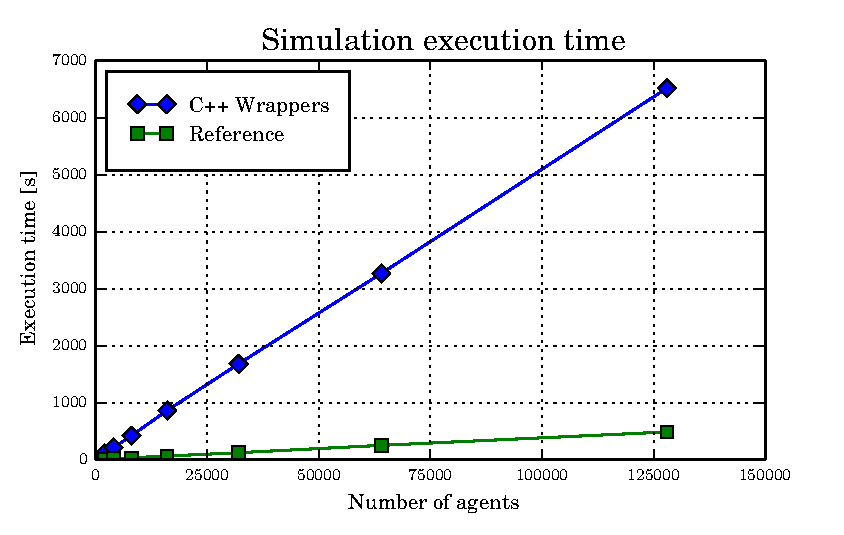
\includegraphics[width=\columnwidth]{graphs/gil-free-perf.eps}
    \caption{Total execution time of simulation with C++ wrappers and full type annotations.}
    \label{fig:gil-free-perf}
  \end{center}
\end{figure}

Before we dive into profiling of this version of code let us have a look at multithreaded
performance of the code. The parallelisation was achieved with use of OpenMP which GCC 4.9.0
supports up to current version (4.0) of the standard.

\subsection{Scalability}\label{subsec:embed-c++-scala}
The issue with scaling simple LERM model is that the simulation itself changes the
location of the agent state in memory. Those underlying data movements make
static scheduling a bad choice, since over time the workload difference between threads
is likely to cause stalls. Therefore we have to settle for dynamic scheduling
of threads. For all of the runs minimal chunk size for the scheduler was set to 50.
Changes were necessary in order to ensure proper scaling of the model with multiple
threads. Those will be outlined shortly. The changes necessary to achieve better
multithreaded scaling did not degrade performance though. It appears that copies
in L1/L2 cache are cheap enough to not have enough visible impact.

To avoid memory allocation in agent update loop we initialise pool of wrappers from
Listing \ref{list:array-adapter-c++} - one for each array in each thread. This way
we avoid additional slowdown and simplify code.

\begin{figure}[H]
  \begin{center}
    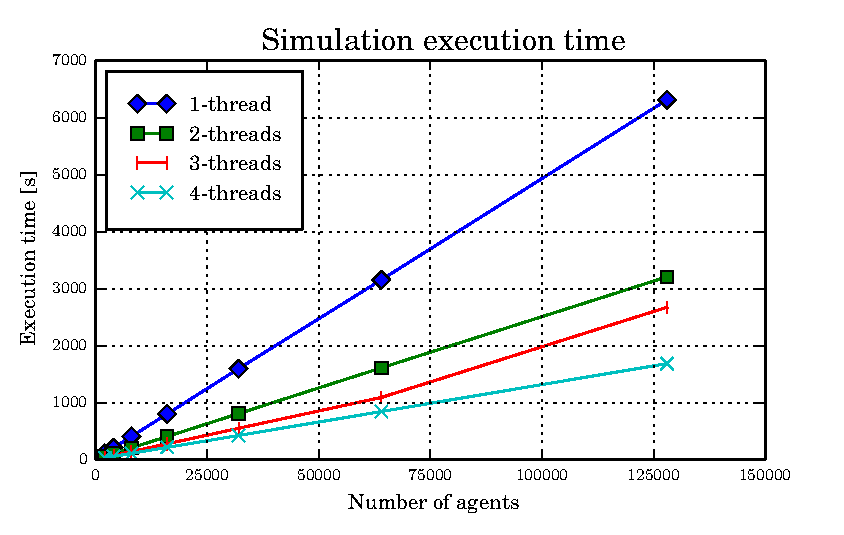
\includegraphics[width=\columnwidth]{graphs/gil-free-multi-4-perf.eps}
    \caption{Execution time for C++ wrappers version for different number of threads.}
    \label{fig:gil-free-multi-4-perf}
  \end{center}
\end{figure}

We achieve very good performance gains - 1.96 times improvement when using two threads,
2.84 when using three and 3.6 when using four. Possible explanation for lack of optimal
scaling is the underlying data movement which prevents CPU to store agent arrays in L1
cache of each core. Whenever an agent will be moved from one core to another it will
have to travel through L3 cache.

\subsection{Further Optimisations}\label{subsec:further-opt}
If we want to achieve results comparable with reference C version we have to once again
defer to profiler for help. There is a presumption that the overhead caused by
\lstinline{std::unordered_map} and \lstinline{std::strin} over \lstinline{float *} and
and \lstinline{char *}.

\begin{table}
  \begin{center}
    \begin{tabular}{|c|c||c|}
    \hline
    Function                                 & Module              & CPU Time               \\ \hline
    \rowcolor{babyblue}
    \_M\_find\_before\_node                  & lerm\_diatom.so     & 58.9617 \\
    \rowcolor{babyblue}
    std::\_Hash\_bytes                       & libstdc++.so.6.0.20 & 42.4008  \\
    \rowcolor{babyblue}
    \_M\_find\_before\_node                  & lerm\_diatom.so     & 35.9007 \\
    \rowcolor{babyblue}
    operator==\textless char\textgreater     & lerm\_diatom.so     & 15.5598 \\
    \rowcolor{babyblue}
    \_\_memcmp\_sse4\_1                      & libc-2.19.so        & 14.8557         \\
    \rowcolor{babyblue}
    \_S\_equals                              & lerm\_diatom.so     & 9.29432 \\
    \rowcolor{babyblue}
    std::\_\_detail::\_Map\_base::operator[] & lerm\_diatom.so     & 9.15494 \\
    \rowcolor{babyblue}
    operator()                               & lerm\_diatom.so     & 8.44585 \\
    lerm\_diatom\_update\_Living\_Diatom     & lerm\_diatom.so     & 8.33352 \\
    \_\_pow                                  & libm-2.19.so        & 5.9977          \\
    \rowcolor{babyblue}
    operator==\textless char\textgreater     & lerm\_diatom.so     & 5.47811 \\
    \rowcolor{babyblue}
    \_S\_equals                              & lerm\_diatom.so     & 4.67876 \\
    \_\_exp                                  & libm-2.19.so        & 4.06897       \\ \hline
    \end{tabular}
    \caption {VTune profile summary for c++ wrapper version.}
    \label{table:vtune-gil-free-profile}
  \end{center}
\end{table}

Quick look at Table \ref{table:vtune-gil-free-profile} shows that it is exactly the case.
The highlighted lines are functions which perform lookup on \lstinline{std::unordered_map}.
Given that the lookup is exhaustive - whole map will be read for each agent update function
call and number of times it is done the overhead seems justifiable. In the end we have
gained convenience of accessing agent fields via natural names instead of integer values.
Hence, only possible way of improving the code further is finding a way of replacing
hash maps with static arrays. This goes against possible extensibility and ease of use since
the code is dependent of memory layout. Furthermore only in the VEW based example we have
detailed knowledge of constants and way agents are allocated. In case of Fluidity-ICOM
the situation is more complicated since only at runtime we will know the layout of agents
in memory and would have to perform substitutions on the fly. In fact we can do exactly that.
In Fluidity-ICOM there is an initial compilation stage at which the memory layout is already
known but before the agent update code has been compiled. We will hook into that process
to achieve better performance. In case of VEW based simple LERM model we will perform one
off substitution of indices.

\section{Removing hash maps}\label{sec:remove-dict}
Once we remove hash maps and use plain C array we should achieve identical performance
to reference C version. In profiler output of previous version there was no other bottleneck
visible.

\begin{figure}[H]
  \begin{center}
    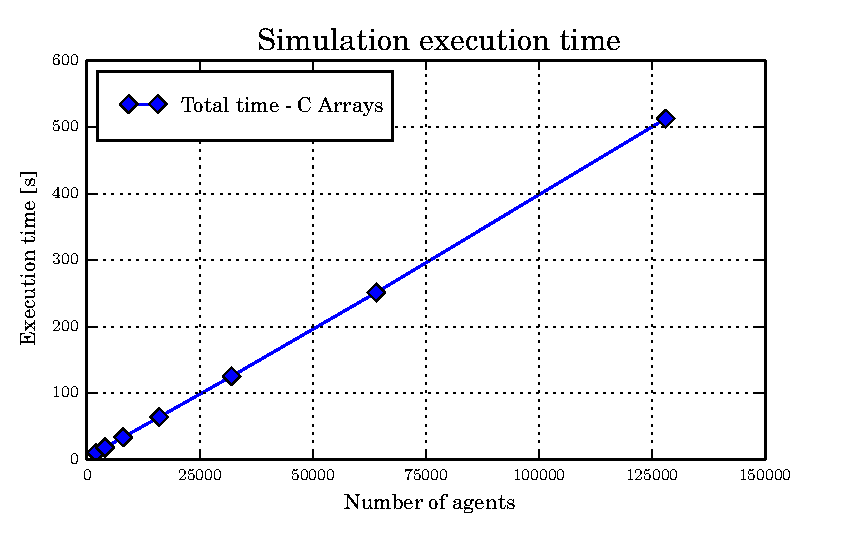
\includegraphics[width=\columnwidth]{graphs/dict-array-perf.eps}
    \caption{Execution time for version with C arrays.}
    \label{fig:dict-array-perf}
  \end{center}
\end{figure}

Figure \ref{fig:dict-array-perf} shows that have managed to achieve the desired result.
The line looks similar to one presented by Figure \ref{fig:master-perf}. Let us have
a look at profiler output.

\begin{table}
  \begin{center}
    \begin{tabular}{|c|c||c|}
    \hline
    Function                             & Module          & CPU Time [s] \\ \hline
    lerm\_diatom\_update\_Living\_Diatom & lerm\_diatom.so & 5.69697      \\
    \_\_pow                              & libm-2.19.so    & 5.3078       \\
    \_\_exp                              & libm-2.19.so    & 3.82439      \\
    getPLayer                            & LERM            & 2.98788      \\
    main                                 & LERM            & 2.15342      \\ \hline
    \end{tabular}
    \caption {VTune profile summary for version with c arrays.}
    \label{table:vtune-dict-array-profile}
  \end{center}
\end{table}

From Table \ref{table:vtune-dict-array-profile} we see that the execution time and
functions which contribute most of it are similar to ones for \ref{fig:vtune-master-perf}.
This is to show that we have eliminated overhead associated with CPython and gained
ability to dynamically load code to our simulation without need of recompiling the program
(the agent update code needs to be compiled though). Furthermore by eliminating the hash
maps we removed the need to wrapper classes thus greatly simplifying the binding code. In
this version the following is sufficient

\begin{lstlisting}[
    caption=Cython binding code when there is no need for array wrappers,
    label=list:cython-bindings-array,
    language=python,
]
cimport lerm_diatom.lerm_diatom as diatom

cdef public void _updateLivingDiatom(float * vars, float * rel, float temp, float vis_irradiance, float * chem) nogil:
    cdef float * chemVals = [temp, vis_irradiance, chem[0], chem[1], chem[2]]
    diatom.update_Living_Diatom(vars, chemVals, rel)


cdef public void _updateDeadDiatom(float * vars, float * rel, float temp) nogil:
    cdef float * chemVals = [temp]
    diatom.update_Dead_Diatom(vars, chemVals, rel)
\end{lstlisting}

In the sample provided by Listing \ref{list:cython-bindings-array}
\lstinline{rel} is used as a return value of the agent. It is allocated before
function call, in C part of simulation, and populated by agent update code to
provide bio-feedback from agent to the environment. Let us have a look at scalability
since after achieving equal single threaded performance multithreading can bring
actual performance gains over reference model.

\subsection{Scalability}\label{subsec:embed-array-scala}
Figure \ref{fig:dict-array-multi-4-perf} shows performance of latest code version
with 1 to 4 threads. The performance gains depend on number of agents the simulation
is running with. While with 4000 agents going from 1 thread to 2 gives 1.65 factor
improvement, for 128000 agents it is already 1.85. Furthermore when the agent update
code is so fast the other non threadable components begin to play part. For 4000 agents
the impact of Particle Management is negligible at 358 ms while for 128000 agents it
is already 17573 ms. If we look only at the agent update code for 128000 agents we
will get speed up factor of 1.92. Similarly for 3 threads it is 2.76 and 3.53 for 4
threads. While if look at the whole program performance we only achieve 2.58 and 3.2 respectively.

Since the speedups are not consistent amongst different agent levels it suggests that
the overhead of data movement (even only to L3) is greater than gain in execution time.
VTune confirms our findings saying that our program is backend bound (computation) and
fully saturates floating point pipeline of the CPU.

Full results with separation for agent update, Particle Management and environment management
can be found in Appendix \ref{appen-ch:bench-results}. For table used to generate this graph refer
to section about threading version with C arrays \ref{appen-subsec:bench-array-multi}.

\begin{figure}[H]
  \begin{center}
    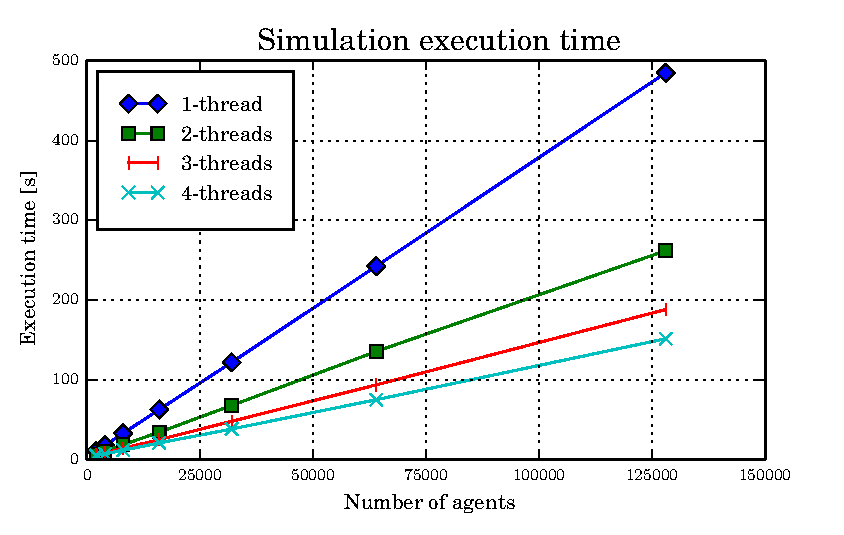
\includegraphics[width=\columnwidth]{graphs/dict-array-multi-4-perf.eps}
    \caption{Execution time for version with C arrays for different number of threads.}
    \label{fig:dict-array-multi-4-perf}
  \end{center}
\end{figure}

\subsection{Cache contention}\label{subsec:cache-contetion}
The VEW based simple LERM model was not made to be threaded. Therefore initial threading
implementation was unnecessarily slow as it was designed for single thread execution.
Here again VTune turned out to be of great use showing places where performance was
deviating from rest of the code.

\begin{figure}[H]
  \begin{center}
    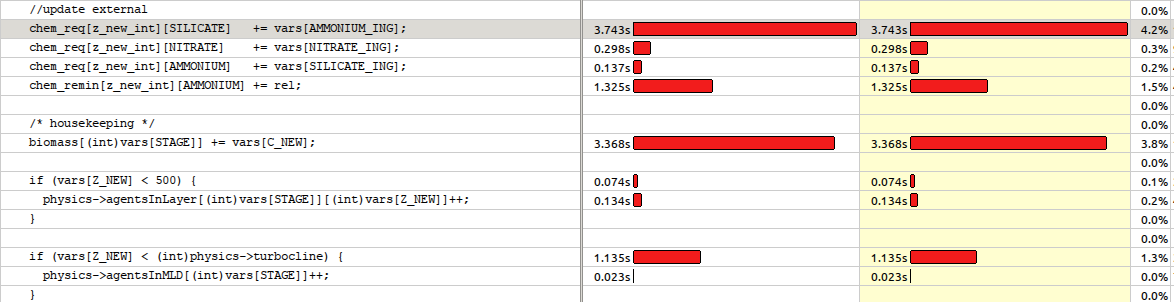
\includegraphics[width=\textwidth,natwidth=1174,natheight=332]{images/cache-cont-before.png}
    \caption{Cache contention on shared environment variables.}
    \label{fig:cache-contention-before}
  \end{center}
\end{figure}

Figure \ref{fig:cache-contention-before} illustrates VTune output for contented lines.
It is clear that something wrong is happening there. To give context to the
values, the complete run took roughly 22 seconds. Writing to the array
should not constitute seconds of running time.

Knowledge of cache architectures is essential to understand the problem. If
other thread tries to write to data which is shared it has to check whether
its copy is still valid. If it is not it has to wait for synchronisation
between the cores caches. If all four cores try to write to same line they
will fight for access and each of them will spend time needlessly waiting
for the data to be written back to L3 cache.

The solution to this problem is to provide per thread copies of environment
variables which will be accumulated at the end of the loop. Additionally
without this change the simulation no longer behaves correctly in multithreaded
version. Since same shared data can be read by multiple threads agents think
they are in a different environment they are actually in. In single threaded
version each of the agents first wrote back its environment changes before
next one proceeded with update. With per thread copies we manage to recover
some of its behaviour but we have made each of agents update in given time step
independent of each other. The reduction step is performed once all of the
living and dead agents have been advanced to the next step. If we want to
allocate thread private data in an array it is essential to ensure that each
of the threads sub arrays does not share a cache line. Due to false sharing the
problem might still persist for small arrays.

\begin{figure}[H]
  \begin{center}
    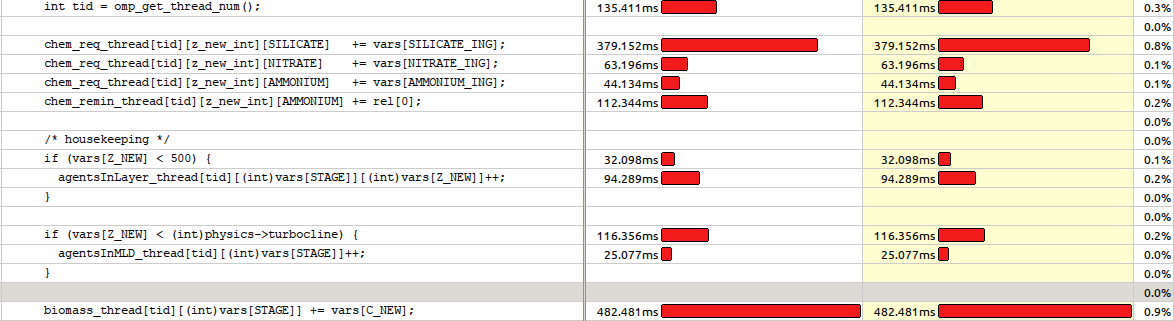
\includegraphics[width=\textwidth,natwidth=1174,natheight=321]{images/cache-cont-after.png}
    \caption{Per thread environment variables}
    \label{fig:cache-contention-after}
  \end{center}
\end{figure}

While all of the penalty will not be eliminated the change manages to give us
4 seconds back from the execution time. More importantly though, with increasing
number of threads the performance would degrade further. Figure
\ref{fig:cache-contention-after} shows behaviour of contentious part of code
after per thread environment variables and reduction phase has been introduced.

More detailed analysis of multithreaded performance of simulation as well as
correctness of the model will be shown in \ref{ch:evaluation}.

\section{Summary}\label{sec:simple-lerm-summ}
In this chapter we have shown how to eliminate performance penalty associated
with using Python and how to avoid GIL and allow threading of the simulation.
Starting with naive embedding using Cython which performed significantly worse.
Then we have begun to add type information to allow Cython to generate efficient
C code. We have changed the way arguments are passed into the function as well
as the way functions are defined. However, that was not enough to achieve
same performance level as reference implementation. In the end we had to
remove convenience of the dictionary and substitute it with pure arrays.
However, since this step is dependent on memory layout at program runtime
we will perform the substitution automatically and allow users specify
their programs with dictionaries. Figure \ref{fig:compared-single-perf} shows
single threaded performance for all of the code versions we had analysed.
We can see that the reference version and version with C arrays overlay
each other.

\begin{figure}[H]
  \begin{center}
    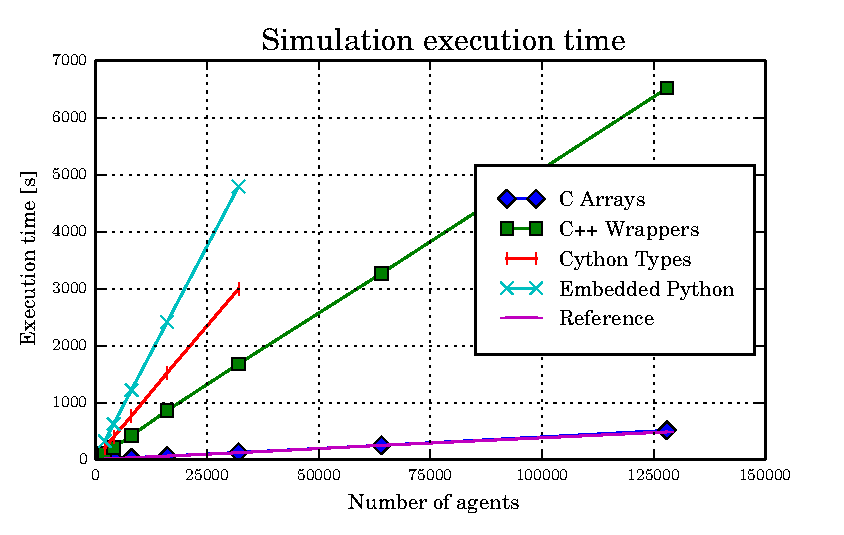
\includegraphics[width=\columnwidth]{graphs/compared-single-perf.eps}
    \caption{Comparison of single threaded execution time for all code versions.}
    \label{fig:compared-single-perf}
  \end{center}
\end{figure}

More detailed analysis of multithreaded performance will be carried out in
\ref{ch:evaluation} where we will see how our program scales for up to 16
threads on 2 CPUs and how data movement and separate caches impact performance.

\chapter{Fluidity Simple LERM Model}\label{ch:thread-fluid}
Some of the design decisions that we have made when working with VEW based
simulation were based on the fact that the target software which would
be using our technique is different and exhibits different properties.
For instance we need dynamic loading since Fluiditiy-ICOM is large
piece of software and fully customisable by the user. Hence, recompiling
it each time is not a possible solution. Secondly we have decided
not to focus on any other parts of the simulation than the agent update.
Being computational fluid dynamics computation software Fluidity is
optimised to handle environment changes efficiently. We only have to consider
performance of variable code supplied by the user. Furthermore Fluidity
already embeds Python for customizing other parts of the runtime, hence,
replacing Python with a different language would have increase amount
of work necessary. Last but not least we have removed dictionaries in favour
of plain arrays to optimise performance. This was dictated by Fluidity-ICOM
configuration specification and ability to rewrite the code on the fly.

\section{Implementation differences}\label{sec:impl-diff}
Fluidity is significantly more sophisticated piece of software than the simple
simulation we have been analysing. While there's benefit to be able to
produce minimal viable product that has the characteristics of the target
software. It speed up analysis and benchmarking significantly. To confirm
that the methodology outline in Chapter \ref{ch:opt-simpl-lerm} is useful we have to
show how to apply it to real simulation software. Fluidity provides the
environment management and scaling. It uses OpenMPI to distribute the
work to multiple machines. Due to its adaptive remeshing it can provide
good trade-off between simulation resolution and performance. As a program
Fluidity is a mixture between C and Fortran therefore we cannot chose
different Python implementation than CPython. Furthermore it already
integrates CPython (PyPy might have been an alternative provided it
had better embedding capabilities). Fluidity reads the configuration from
xml file supplied by the user. For purpose of ecosystem modeling the
configuration contains the code that defines functional groups in the
simulation, specifies the initial conditions and types of fields that are
present in the simulation. The code that will be run by the simulation has
to be read from the file and compiled to then be executed for each of the agents.
Furthermore the results of the agent code have to be passed to the Fortran
physics engine to determine changes in the system.

\section{Compiling agent code}\label{sec:compl-agent-code}
Work on Fluidity integration was not completed as of writing this section. The
section outlines the work done so far and the challenges that had to
be overcome. Remaining pieces are porting of Fluidity-ICOM Python
API for agents to not use Python C/API.

When working with the simple VEW based simulation we had the convenience of
non changing location of code and ability to change the agent update code
freely. With Fluidity we can no longer assume this. The agent code provided
by the user can be arbitrary Python code, i.e. import other modules. Needless to say we will
have to introduce constraints on the type of code that the user can
write. We have to have direct C/C++ translation in order to achieve GIL
free execution. Throughout the development process Python's distutils have
been used for compilation of Cython extensions. While distutils are
easy to configure they can only operate on files. Therefore
we construct the structure of the module on the fly while reading the
configuration file. The additional complication comes from the fact
that the compiled module with agent update and initialisation code has
to be importable from Python.

Hence, users cannot use non GIL-free code when defining their agents
behaviour, i.e. type annotations have to be provided. Fluidity-ICOM
will generate proper Cython header files to expose the C
style functions from agent code. We rely on the fact that
Cython generated modules expose pure C/C++ functions that can be used
even if the module has not been properly initialised from Python's
point of view. The glue code that provides interaction between
user supplied code and simulation engine is responsible for setting
up the user provided code in the module and importing it. We use
C++ part to transform the code, only after the user
supplied code has been compiled into a module the linking module
is initialised - at this point Python will populate the symbols
used in the module. This works due to the fact that C/C++ do not
need to know definition of the function to compile the program that uses it
but only the prototype is necessary. Only when the module is
initialised the code is loaded and function symbols point to executable
code. Before code is compiled it undergoes transformation to replace
dictionary accesses to environment and agent variables with array indices.


\chapter{Evaluation}\label{ch:evaluation}

We had set out to optimise performance of naive Python embedding in C
applications. In particular we wanted to achieve scalability. Since
GIL is a feature of CPython that is difficult to remove a scheme
to avoid it has been shown. Achieving multithreaded execution would
not be useful if the single thread performance was significantly worse.
Therefore with help of Cython we have shown how pure Python code can
be type annotated to provide C level speeds.

We had talked about implementation details and performance
improvements resulting from them in \ref{ch:opt-simpl-lerm} and have
given a sketch of implementation into large scale simulation engine
Fluidity-ICOM in \ref{ch:thread-fluid}. What we are going to look
at now is how the changes impact the characteristic properties
of the model.

Further threading results will shown to illustrate the performance
on multi CPU architectures. Results in this section all come from
benchmark results from machine with 4 Sandy Bridge CPUs
(8 cores each - E5-4650 @ 2.7 Ghz) with 500 GB of RAM. However,
only 2 CPUs have been used as mentioned in Section \ref{sec:exp-setup}.
We will use results from both machines to compare the architectures and
try to understand what type of low level features affect the execution
time of the simulation.

Figure \ref{fig:target-initial-comp-perf} illustrates the gap we had
closed with all of the modifications to the code. The initial version
also had scalability limitations due to GIL which we had to overcome.
On the other hand the reference C version does not provide modular
code loading. Whole simulation code has to be recompiled if changes
to agent behaviour are necessary. With large simulation software
this approach is not feasible as the configuration is only known at
runtime. Recompiling whole simulation application between changes
wouldn't yield good user experience and introduce unnecessary overhead.

\begin{figure}[H]
  \begin{center}
    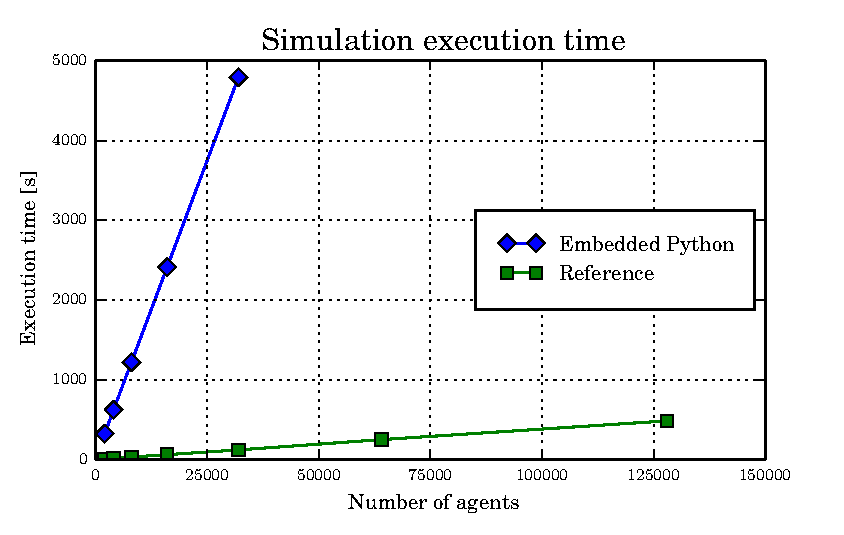
\includegraphics[width=\columnwidth]{graphs/initial-target-perf.eps}
    \caption{Performance difference of reference and initial code version}
    \label{fig:target-initial-comp-perf}
  \end{center}
\end{figure}

\section{Reference version scalability}\label{sec:ref-c-scala}

For completeness the reference C version was also parallelised and benchmarked
to provide baseline for comparisons. What we can notice from the Figure
\ref{fig:master-perf-multi-16} is the nonlinear scaling with increasing number
of threads. Knowing performance constraints of our simulation helps explain
the phenomenon. Throughout the execution of the program the most of work
is coming from reading agent parameters and performing floating point operations
on them. Thus, as confirmed by profiler, the execution is limited by FLOPS
performance of CPU. Any CPU cycle spent not executing arithmetic operations
is a loss of performance. With more than eight threads we have begun using
2 CPUs which do not share caches. If for single CPU an L3 cache hit instead
of L1 (due to data movements) is a bottleneck, the main memory will be even
bigger performance hit.

\begin{figure}[H]
  \begin{center}
    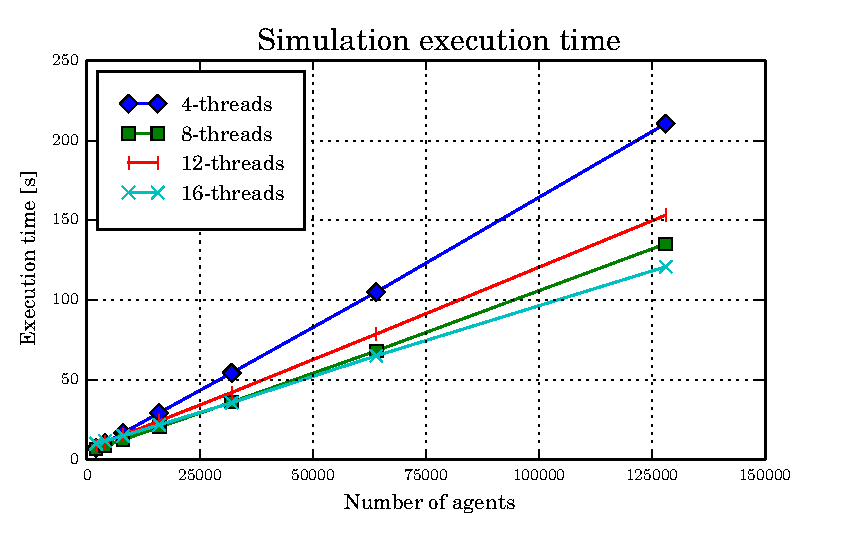
\includegraphics[width=\columnwidth]{graphs/master-perf-multi-16.eps}
    \caption{Performance of reference C version for up to 16 threads}
    \label{fig:master-perf-multi-16}
  \end{center}
\end{figure}

\section{Model Correctness}\label{sec:model-correct}

\section{Biomass}\label{subsec:model-correct-bio}
At the beginning of Chapter \ref{ch:opt-simpl-lerm} we have seen characteristic
biomass and agent curves in the simulation. For the result to be correct
those two should remain consistent throughout with that version. From Figure
\ref{fig:bio-single-comp} we notice that the changes have altered the bloom
cycle of plankton. First two versions which still relied on Python semantics
with small Cython additions show largely similar curves (identical in case
of typed cython version). Further changes, however, changed the numerical results
of the simulation. This suggests that along the way the agent update or its
integration with rest of simulation code was altered in incompatible way.
Despite this fact, the simulation is still stable and has similar number of
agents as Figures \ref{fig:ag-single-comp} and \ref{fig:ag-multi-comp} show.
The change must have been introduced when Python dictionaries have been
removed. Further investigation has to be carried out to confirm where the difference
comes from. The good part is that the two versions C and C++ are consistent with
each other which reduces the potential sources of error.

\begin{figure}[H]
  \begin{center}
    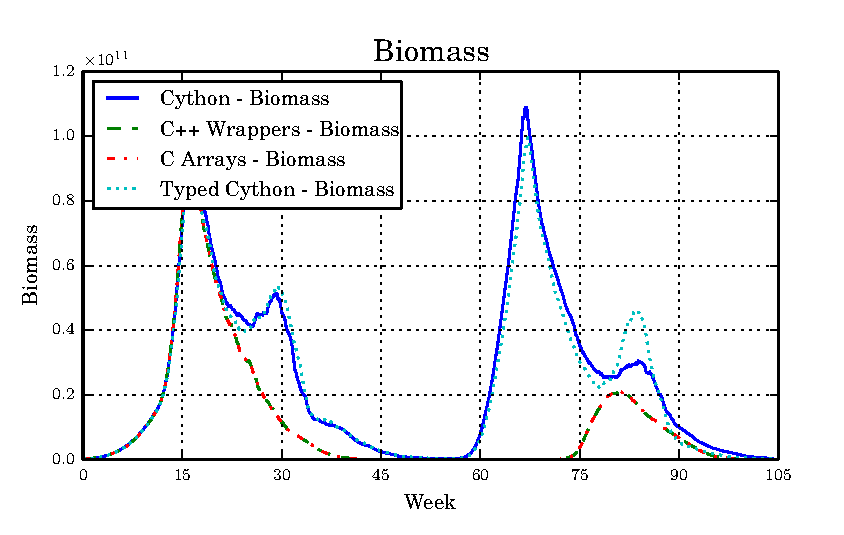
\includegraphics[width=\columnwidth]{graphs/bio-single-comp.eps}
    \caption{Biomass comparison between different code versions for 1 thread.}
    \label{fig:bio-single-comp}
  \end{center}
\end{figure}

For multithreaded case we had introduced thread local copies of environment. Therefore
at beginning of each iteration all of the agents are presented with same environment
which is only updated at the end. The previous behaviour updated the environment at
the end of each agent update. This introduces changes in the results of the simulation.
The threaded reference C version will be used as a baseline for comparison as we have
not changed the agent update code and it posses same biological characteristics as
its single threaded version. Figure \ref{fig:bio-multi-comp} illustrates the biomass
for multithreaded versions of the simulation for eight threads. The initial bloom
period remains unaffected. The reference version, however, has similar features
to its single threaded version that others don't. There's slight bump after
bloom peak and second bloom period with bump after peak. In case of C and C++ versions
there's no bump after bloom periods.

\begin{figure}[H]
  \begin{center}
    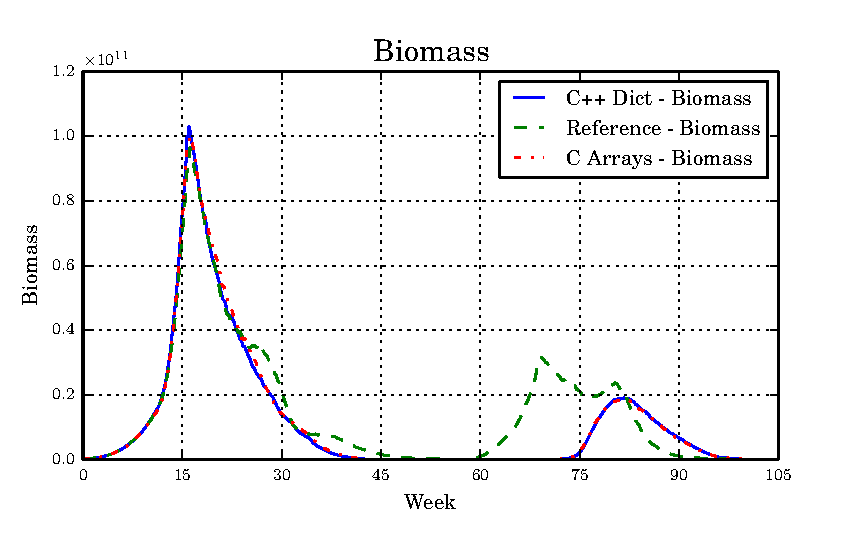
\includegraphics[width=\columnwidth]{graphs/bio-multi-comp.eps}
    \caption{Biomass comparison between different code versions for 8 threads.}J
    \label{fig:bio-multi-comp}
  \end{center}
\end{figure}

\section{Agent count}\label{subsec:model-correct-agent}
Other characteristic feature of our simulation is the number of agents. As the
simulation implements an LE metamodel the number of agents changes to provide
appropriate sampling resolution and computational complexity. Therefore the
execution time is mostly dictated by number of agents. If the numerical
correctness was not preserved this does not mean that our methodology in
principle will not lead to speedup. From Figures \ref{fig:ag-single-comp} and
\ref{fig:ag-multi-comp} we can see that the number of agents remains very
similar throughout for the versions which report different biomass of the
ecosystem. What is more the biomass change had caused increase in the number
of agents in later stages. As a result those versions of the simulation had
to perform more updates and should take more time to execute. Thus in principle
the speedup achieved in version with C++ wrappers as well as C arrays could have
been greater.

\begin{figure}[H]
  \begin{center}
    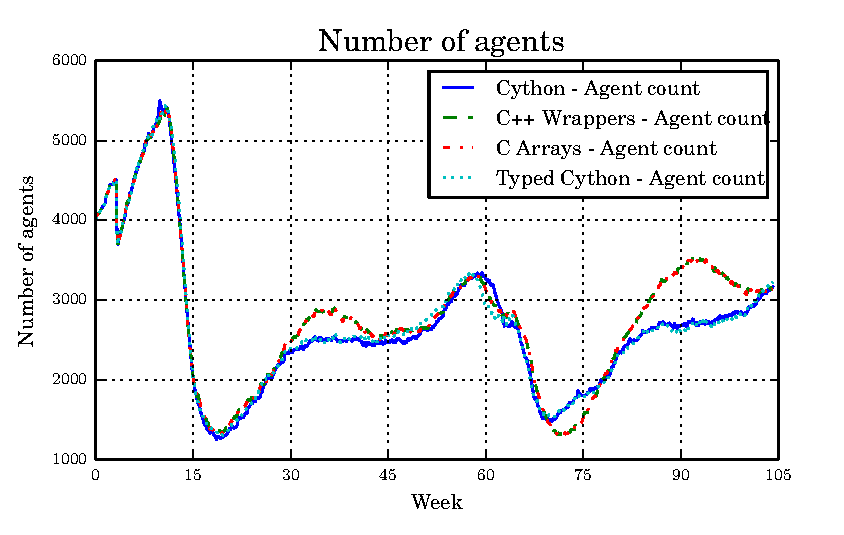
\includegraphics[width=\columnwidth]{graphs/ag-single-comp.eps}
    \caption{comparison of number of agents between different code versions for 1 thread.}
    \label{fig:ag-single-comp}
  \end{center}
\end{figure}

\begin{figure}[H]
  \begin{center}
    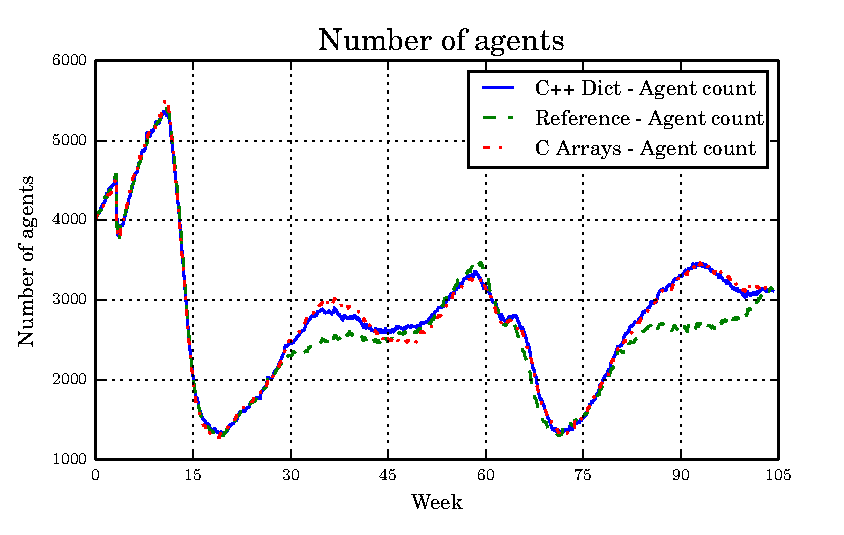
\includegraphics[width=\columnwidth]{graphs/ag-multi-comp.eps}
    \caption{comparison of number of agents between different code versions for 8 threads.}
    \label{fig:ag-multi-comp}
  \end{center}
\end{figure}

\section{Parallel execution via C++}\label{sec:para-c++}
To illustrate the importance of single thread performance the version with C++ wrappers
had been benchmarked for up to 16 threads. The results are shown in Figure \ref{fig:gil-free-multi-16-perf}.
In \ref{sec:embed-c++} we had seen that this version is roughly \emph{11 times} slower
than the reference version. If we achieve linear scaling with number of threads
then with 11 threads the performance of the two versions should be equal. Figure
\ref{fig:gil-free-multi-16-perf} illustrates that it is not the case. There is roughly
6 times speedup over single threaded version for 8 threads and only factor of 9 for 16
threads. This is due to nature of memory accesses and data transfers across CPUs.
Parallelising program is not a trivial exercise and improvements in sequential version
of the program should be attempted first. Running with 16 threads this code version was
still 60\% slower than reference C implementation running with 1 thread.

\begin{figure}[H]
  \begin{center}
    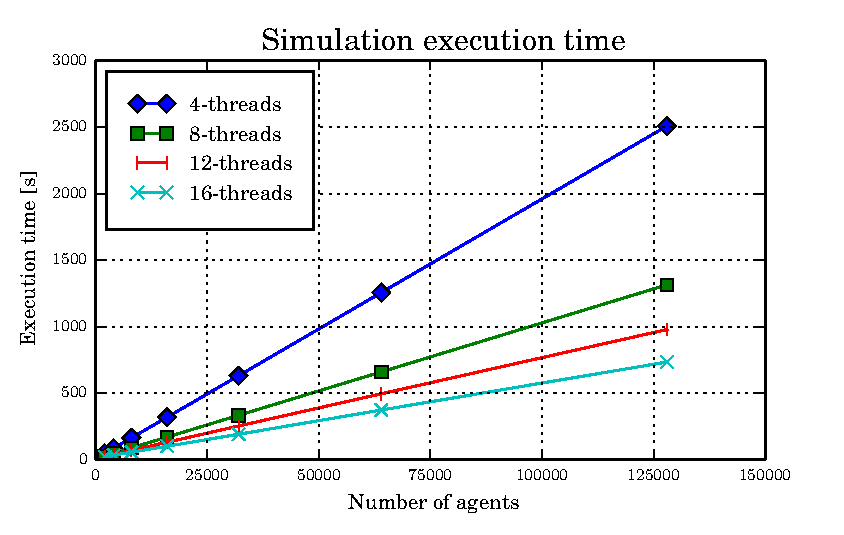
\includegraphics[width=\columnwidth]{graphs/gil-free-multi-16-perf.eps}
    \caption{Performance of C++ Wrapper version for up to 16 threads.}
    \label{fig:gil-free-multi-16-perf}
  \end{center}
\end{figure}

\section{Using C arrays}\label{sec:array-use}
We are going to have a deeper look at the performance difference between final
version of embedding code that uses C arrays for agent variables and the reference
C version. Figure \ref{fig:dict-array-multi-16-perf} shows same trend for
4, 8 and 12 threads as the parallelised reference version. However, there is
a significantly worse result for 16 threads. As the results throughout suggest
that there is no visible difference between those two code versions we have
reason to believe that this is an anomaly in the experiment. Likely a scheduled
job triggered which interfered with running of the simulation. Figure \ref{fig:speedup}
confirms this hypothesis showing that up to 15 threads both code versions have
same speedup curves. This should lead us to conclude that with minor difference the
both code versions perform in the same fashion. Larger speedup factor achieved
by the version with embeddable code is due to slightly worse single thread performance.
However, the final performance for 15 threads (when we ignore 16 thread anomaly) is better
for the version with embeddable code. When it comes to the speedup curve we see steady
growth up to 8 threads where we get factor of 5 improvement. The trend line breaks as
soon we cross 1 CPU boundary. Due to need to move data across CPUs and larger latency
of those transfers than L3 cache hits the benefit of more computational power due to
larger number of threads is offset by memory synchronisation. We will have a look
at why it happens exactly in \ref{subsec:mult-cpu-arch}.

\begin{figure}[H]
  \begin{center}
    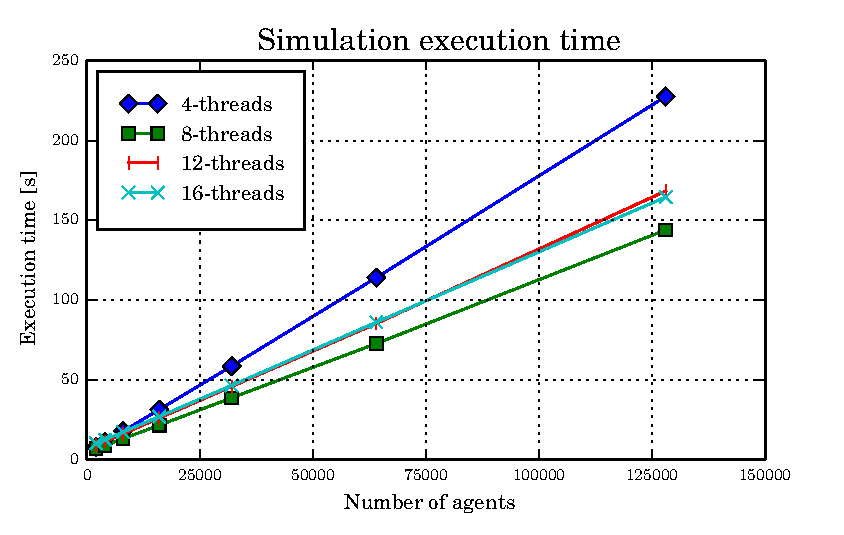
\includegraphics[width=\columnwidth]{graphs/dict-array-multi-16-perf.eps}
    \caption{Performance of C Arrays version for up to 16 threads.}
    \label{fig:dict-array-multi-16-perf}
  \end{center}
\end{figure}

\begin{figure}[H]
  \begin{center}
    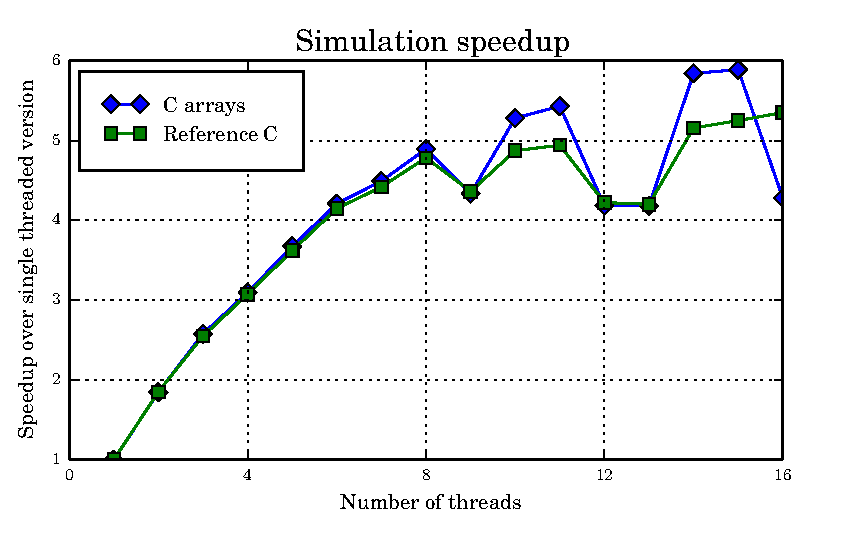
\includegraphics[width=\columnwidth]{graphs/speedup.eps}
    \caption{Speedup for multiple threads over single threaded version.}
    \label{fig:speedup}
  \end{center}
\end{figure}

\subsection{Multi CPU architectures}\label{subsec:mult-cpu-arch}
When working with a single CPU one can assume that increasing number of threads
will likely bring performance improvement as most of the data is shared between
threads via Last Level Cache (usually L3). Therefore there is no significant
performance hit when moving data around. While it will be noticeable, i.e.
it will prevent us from achieving linear scaling it is something that can
be solved by ensuring each threads works on its local copy of the data. With
multi CPU architectures the communication overhead becomes greater. It is still
possible to provide a local copy for each thread to preserve locality, however,
the eventual movement incurs greater penalty. In case of Intel's Sandy Bridge
EP architecture that was used for multi CPU benchmarks the CPUs are connected
by Quick Path Interconnect (QPI) which has lower throughput and greater latency
than local caches. The connections between CPUs are shown on Figure
\ref{fig:sandy-bridge-ep-arch} In principle it might be possible to exploit the
knowledge about the CPU the data currently resides and only move it in the
scope of it. Unfortunately OpenMP, used to achieve parallelisation, does not
provide such facilities.

\begin{figure}[H]
  \begin{center}
    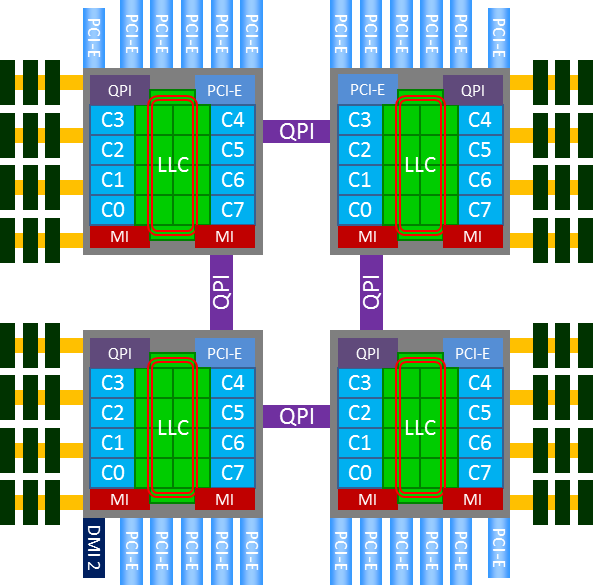
\includegraphics[width=0.7\textwidth,natwidth=593,natheight=585]{images/SandyBridgeEP4c.png}
    \caption{Memory connections in Sandy Bridge EP architecture}
    \label{fig:sandy-bridge-ep-arch}
  \end{center}
\end{figure}

\subsection{Sandy Bridge vs Haswell}\label{subsec:sb-vs-haswell}
Since we had carried out tests on two different architecture we can use our
simulation as a benchmark for architectures and see how much of an improvement
Haswell is in term of performance. Sandy Bridge based machine has visibly
lower performance even when the clock difference is factored. The Haswell
machine runs at 3.4 GHz which is 26\% more than 2.7 GHz that the Sandy Bridge
runs at. However, the benchmark results show difference in range of 45-50\%
for same workload. It suggests that Haswell has some micro architecture
features that help our simulation achieve better timings. VTune profiles
come to play again. The simulation code is bound by the performance
of floating point pipeline and memory throughput. To understand the difference
between the two architectures we refer to the articles about
Sandy Bridge (\cite{SandyBridgeArch}) and Haswell (\cite{HaswellArch}) design. There are two
differences that stand out when comparing the architectures with our code in mind.
First of all we have to note that Sandy Bridge caches are fully pipelined
and running at the clock speed of the CPU itself. This makes them fast since
there is no frequency boundary. On the other hand Haswell has three different
clocks on the socket and CPU and LLC do not operate at the same frequency.
However, Haswell has larger throughput and can sustain 256-bit loads and a
256-bit store every cycle. In contrast, Sandy Bridge can only support two
128-bit reads and a 128-bit write per cycle. Given how dependent on data
movements the performance is this seems to be an important feature. With our
code performing large number of data lookups this difference seems to be
significant. The presumption comes from the fact that the benefit Haswell
has increases when going from 1 thread to 4 (from 45\% to 50\%). The more
important part though are Fused Multiply Add (FMA) and lower latency floating
point add. The FMA instructions reduce latency of operations like
$c = a \times b + c$ from 8 cycles in Sandy Bridge to 5 in Haswell.
Additionally the forward infrastructure has been widened hence,
Haswell CPUs can forward results more bytes thus reducing latency as
forwarding does not involve going back to cache for data.
Profiling output of the simulation code on Sandy Bridge EP
architecture would be necessary to confirm the presumption. There is
definitely something more involved happening as Haswell only promises
roughly 10\% improvement for same clock speeds. Our simulation gets
visibly larger boost from changing the underlying architecture.

\section{Load balancing}\label{sec:eval-load-balance}
Through out the benchmarking process the OpenMP scheduler was set to ``runtime''
and configured to ``dynamic,50'' as a value that was found to be good enough
during quick testing. In order to verify that we had chosen right value
and there is no possible improvement due to changes in the way data is
allocated to threads benchmarks of different scheduler settings were carried
out. For those experiments the number of agents was set to 64000 and 4 threads
running on i7 4770 @ 3.4 GHz. The upper bound was set to number of agents
divided by number of threads as this is maximal number that will ensure that
all of the threads are running. From Figure \ref{fig:schedule-high} we see
that size of chunk for scheduler can have a significant impact of performance.
However, it proved of no use when looking for optimal value. The tests had
been rerun concentrating on lower end of value range. Figure \ref{fig:schedule-low}
shows the performance for chunk sizes from 0 to 100. There is rapid performance
improvement that levels off around 10 and decreases steadily until 40. After
that the execution time fluctuates and there's no clear minimum. For this
graph it is 72 but only by a small margin as in 40-100 range the execution
times do not vary by more than 0.5s. Therefore we can conclude that setting
chunk size to 50 was a good choice and there is no visible improvement that
could have been achieved by choosing a different value.

\begin{figure}[H]
  \begin{center}
    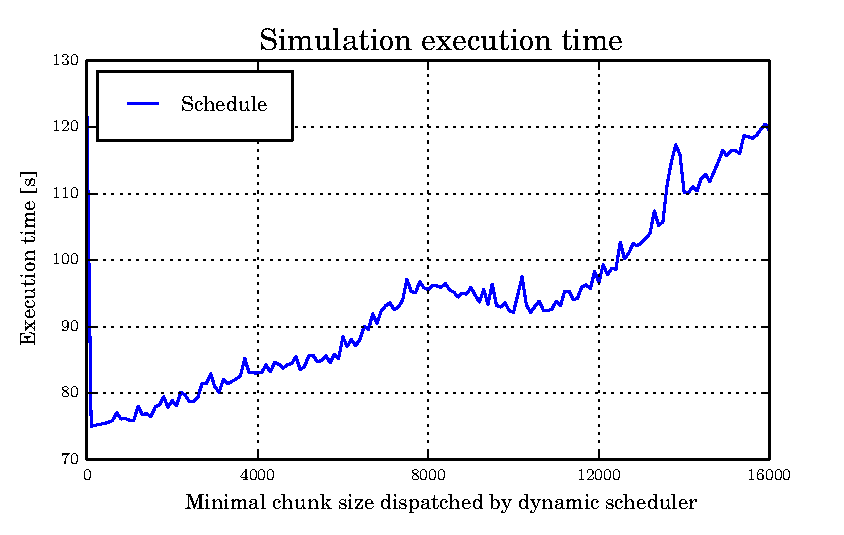
\includegraphics[width=\columnwidth]{graphs/schedule-high.eps}
    \caption{Performance of C Array version for 64000 agents for different scheduler setting.}
    \label{fig:schedule-high}
  \end{center}
\end{figure}

\begin{figure}[H]
  \begin{center}
    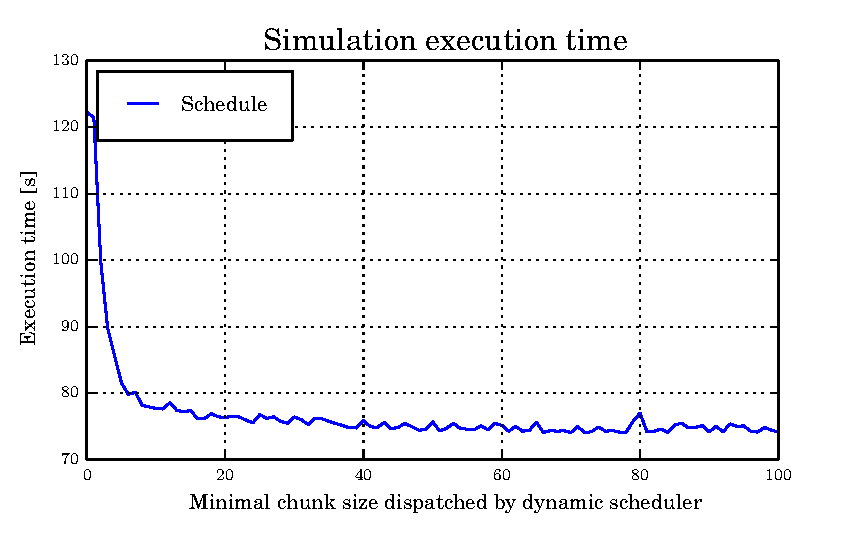
\includegraphics[width=\columnwidth]{graphs/schedule-low.eps}
    \caption{Performance of C Array version for 64000 agents for different scheduler setting.}
    \label{fig:schedule-low}
  \end{center}
\end{figure}

\section{Fluidity}\label{sec:fluid-appcl}
Since the work on integrating the outlined optimisation methodology had
not been finished there are no benchmark results to present and compare.
The technique is promising as it does not involve rewriting the application
completely and allows to simply swap Python for something that performs
better. Fluidity-ICOM code performs many data copies to convert data
to Python format which our implementation avoided from the start. Therefore
there is potential for even larger performance gains when performing
agent update loop. With Fluidity-ICOM being able to run simulations
at arbitrarily large machines (Fluidity itself performs partitioning
of the data via OpenMPI) it then can be used to recreate complicated
experiments and provide a tool that is as capable as VEW. Furthermore
as VEW uses Planktonica to model specification the types of models that
it can represent are limited by the expressiveness of the tool. With
Cython as a definition language the possibilities are unlimited  since
we are using a fully fledged programming language.

\chapter{Conclusion}\label{ch:concl}
Throughout the work we have demonstrated how Python can be optimised to match
C performance. To demonstrate the effectiveness of the approach an
ocean ecology simulation had been used. The report outlines the iterations
that uncover next bottlenecks and show how abstraction layers come work
against performance of the application. Effectively we arrive at a version
that is as fast as reference implementation that has been used as a baseline.
What our solution achieves is familiarity of syntax. What the user writes
is not far from Python though it is not technically Python. Additionally
we achieve dynamic code loading and avoid recompiling whole simulation
with every change to user supplied code.

\section{Summary}\label{sec:summary}
We had begun with embedding Python directly in the application. Instead of
using Python C/API directly we had employed Cython to generate appropriate
functions thus we had only write the code that was responsible for data
conversion. The boilerplate involved when defining Python modules had
been taken care of for us. The naive embedding while easy to implement
and not requiring any code compilation was extremely slow. Even though
the implementation avoided data copies the slowdown was by factor of \emph{35}.
What is more naive embedding entails GIL when executing the code. The
main objective of this project was to combine Python embedding and
parallel execution. Once the initial setting and performance characteristics
of the program had been understood we had set out to optimise the performance
and provided true parallel execution.

The strategy for achieving C level performance concentrated on one idea -
avoid using Python interpreter as it is unable of generating efficient
machine code. First types for variables used throughout Python code had
been defined. That operation had cut down the penalty in half to roughly
\emph{21} factor slowdown. Next step was to avoid using Python dictionaries
while preserving name based access to agent's variables. This involved
recreating wrapper created in Python in C++. As a result of replacing
all of the code with typed versions and C++ containers instead of Python
ones reliance on Python at runtime had been removed. This version while
still \emph{11} times slower had the ability to execute on multiple threads.
We have seen how the code scales. Nonetheless due to non linear scaling
and significant single threaded performance slowdown this version was
still not adequate for use in larger systems.

The last step was to replace C++ containers and remove name based access
to agent's variable. By using plain C arrays we had achieved performance
levels of reference version while maintaining the ability to load code
dynamically at runtime. Furthermore compatibility with Python had been
preserved if multithreaded execution and performance are not a concern.

We had looked at how the code scales and whether the simulation produces
the same output. The code scales quite well when only one CPU is used.
The non linear performance gain from larger number of threads suggests
that the workload should be increased to achieve better efficiency.
However, with multiple CPUs and inter CPU communication the performance
benefit is non obvious. Since the simulation moves the data around
due to development of agents the data layout cannot be fixed and
latency of moving data around eliminates performance benefits coming
from larger number of execution units.

Finally sketch of implementation in Fluidity-ICOM had been outlined.
This report came as a result of its performance drawbacks and it
would be interesting to see improvements presented approach would
give. As Fluidity is fully parallelisable the simulation should
scale to very large models.

\section{Related Work}\label{sec:related}
The approach outlined in this report is not the only possible one to
achieve thread level parallelisim in Python. Other projects present
more universal approaches, however, none of them solves the problem
of CPython compatibility and CPU bound tasks. As such while the work
does not present any new piece of software it outlines how existing
software, i.e. Cython can be used to speed up Python while providing
similar syntax.

\subsection{PyPy Software Transactional Memory}\label{subsec:pypy-stm}
PyPy is the most mature alternative. It had become known in Python
world for targeting CPython compatibility while speeding up single
threaded execution considerably due to introduction of JIT compiler
to the interpreter. Regardless the code itself still has to obey
GIL as it has to be compatible with CPython. Recently, however,
PyPy developers are working on Software Transactional Memory (STM)
to allow multithreaded execution of arbitrary Python code without
removing the GIL.

The idea behind STM is to give each thread its own address space and
create illusion that it is executing on its own and has complete
control of memory. The interpreter is then responsible for intercepting
calls to GIL sensitive regions and allow only one thread at once into
the area. When multiple threads try to acquire GIL at the same time
snapshot of their state is taken and then they compete for the lock.
One of the threads will acquire it and continue execution, while
others will be rolled back to their snapshotted state and replayed
from there. There is an obvious contention problem for certain
workloads. The system might not scale well for large number of
threads. However, given how deeply GIL is entrenched in the Python
execution model it seems to be the only viable alternative.

\subsection{PyParallel}\label{subsec:pyparallel}
PyParallel is another project which wants to preserve CPython compatibility
while allowing multithreaded execution. The project is aimed at I/O and
network operations as it assumes complete separations of executing
threads. The child threads spawned by a master thread are given only
read access to memory. If communication is necessary with the main
thread the implementation provides simple snapshotting techniques
similar to STM but not so sophisticated. The implementation works
by replacing CPython GIL acquire and release routines and replacing them
with own implementations that resolve multiple access conflicts. This
approach while extremely successful for event oriented architecture
where process needs short lived workers to handle a request will
likely not scale for CPU intensive tasks.

\subsection{Jython and IronPython}\label{subsec:other-python-impl}
The last of related projects are Python interpreters written in languages
that provided real garbage collectors. Jython is Python implementation on
top of JVM and IronPython uses C\# Dynamic Language Runtime provided by
.NET. Both of the runtimes provide real parallelism through virtual machines
and since they are not using reference counting for garbage collection
they are not susceptible to GIL. While they fit the performance characteristics
for our application they are highly dependent on the runtimes they work on.
Therefore it is not possible to easily embed Jython or IronPython outside
of JVM based applications or .NET respectively. Last but not least they
do not provide binary compatibility between CPython, hence, its extensions
cannot be used. All in all those implementations are useful for specific
projects where Python is necessary and JVM or .NET is already being used.

\section{Future Work}\label{sec:future}
First possible extension of work presented here is to finish implementation
in real world system like Fluidity-ICOM and prove that it is actually
useful to the users. We are changing slightly the language that is being
used hence usability investigation would prove extremely useful.

While Cython is not an interpreter itself but only an optimising compiler
it would be great to see tighter integration between the two. Cython
can produce Python compatible extension that can also have C interface.
Why not provide Python interpreter with compilation capabilities directly.
It does not have to be a full scaled JIT compiler but something that would
analyse the code being executed, perform type inference or use types provided
by user to optimise the module code and substitute it at runtime upon loading.
Since Cython provides function decorators to specify types the code could
be compatible with pure Python. This would work like \lstinline{pyximport}
with a boost where an attempt at type inference would be made and it would have
been integrated directly into language runtime without the need to explicitly
indicate that we might be importing Cython modules.

Cython's main limitation is the fact that it extends Python's syntax and as
such some of the created code will not be compatible with CPython's interpreter.
By providing compatibility at language level there would be no need to specify
whether the module should be optimised or not and whether it has any forbidden
Python syntax. Once again it is an argument to integrate Cython's capabilities
directly into Python language to allow optional type specifications.

Last but not least, the holy grail of Python multithreading, would be CPython
implementation without GIL and with JIT compilation capabilities. Thus removing the need
for direct compilation all together. This would entail creating a piece of
software comparable with sophistication and complexity to JVM and .NET which
is not likely to happen without direct need for such solution.

% To add something to the bibliography, look for the "import into BibTex"
% thingy on google scholar, and add the stuff into refs.bib.
\bibliographystyle{plainnat} \bibliography{References}

\begin{appendices}
\chapter{Complete benchmark results}\label{appen-ch:bench-results}
\section{Reference C version}\label{appen-sec:bench-ref-c}

\begin{table}[H]
  \begin{center}
    \begin{tabular}{|c||c||c|c|c|}
    \hline
    Number of agents & Total [ms] & Update [ms] & PM [ms] & Env [ms] \\ \hline
    2000             & 10367      & 8949        & 201     & 1117     \\
    4000             & 17794      & 16243       & 336     & 1115     \\
    8000             & 32749      & 30901       & 630     & 1118     \\
    16000            & 62708      & 60207       & 1279    & 1120     \\
    32000            & 121979     & 118034      & 2720    & 1122     \\
    64000            & 251018     & 242488      & 7230    & 1180     \\
    128000           & 486010     & 467940      & 16822   & 1139     \\ \hline
    \end{tabular}
    \caption {Reference C version}
    \label{table:append-reference-timings}
  \end{center}
\end{table}

\subsection{Threading}\label{appen-subsec:bench-ref-c-multi}
\begin{table}[H]
  \begin{center}
    \begin{tabular}{|c||c||c|c|c|}
    \hline
    Number of agents & Total [ms] & Update [ms] & PM [ms] & Env [ms] \\ \hline
    2000             & 9931       & 8514        & 200     & 1117     \\
    4000             & 16974      & 15421       & 337     & 1117     \\
    8000             & 30795      & 28949       & 628     & 1118     \\
    16000            & 59341      & 56839       & 1282    & 1119     \\
    32000            & 115373     & 111407      & 2744    & 1121     \\
    64000            & 228939     & 221410      & 6300    & 1126     \\
    128000           & 460029     & 441934      & 16851   & 1138     \\ \hline
    \end{tabular}
    \caption {Reference C version, thread local variables, 1 thread, i7 4770}
    \label{table:append-reference-timings-1-thread-line}
  \end{center}
\end{table}

\begin{table}[H]
  \begin{center}
    \begin{tabular}{|c||c||c|c|c|}
    \hline
    Number of agents & Total [ms] & Update [ms] & PM [ms] & Env [ms] \\ \hline
    2000             & 6691       & 4658        & 210     & 1713     \\
    4000             & 10411      & 8242        & 344     & 1714     \\
    8000             & 17875      & 15395       & 653     & 1715     \\
    16000            & 32606      & 29483       & 1297    & 1714     \\
    32000            & 62333      & 57743       & 2765    & 1713     \\
    64000            & 122361     & 114219      & 6310    & 1718     \\
    128000           & 246724     & 228165      & 16707   & 1729     \\ \hline
    \end{tabular}
    \caption {Reference C version, thread local variables, 2 threads, i7 4770}
    \label{table:append-reference-timings-2-thread-line}
  \end{center}
\end{table}

\begin{table}[H]
  \begin{center}
    \begin{tabular}{|c||c||c|c|c|}
    \hline
    Number of agents & Total [ms] & Update [ms] & PM [ms] & Env [ms] \\ \hline
    2000             & 5485      & 3401       & 217    & 1753    \\
    4000             & 8097      & 5871       & 355    & 1756    \\
    8000             & 13311     & 10775      & 665    & 1753    \\
    16000            & 23787     & 20587      & 1332   & 1750    \\
    32000            & 44685     & 39974      & 2840   & 1752    \\
    64000            & 87600     & 79179      & 6533   & 1766    \\
    128000           & 176652    & 157819     & 16938  & 1765    \\ \hline
    \end{tabular}
    \caption {Reference C version, thread local variables, 3 threads, i7 4770}
    \label{table:append-reference-timings-3-thread-line}
  \end{center}
\end{table}

\begin{table}[H]
  \begin{center}
    \begin{tabular}{|c||c||c|c|c|}
    \hline
    Number of agents & Total [ms] & Update [ms] & PM [ms] & Env [ms] \\ \hline
    2000             & 4995      & 2865       & 224    & 1791    \\
    4000             & 7107      & 4835       & 366    & 1791    \\
    8000             & 11269     & 8677       & 686    & 1790    \\
    16000            & 19616     & 16342      & 1368   & 1789    \\
    32000            & 36353     & 31553      & 2890   & 1789    \\
    64000            & 70397     & 61860      & 6626   & 1789    \\
    128000           & 142544    & 123327     & 17287  & 1797    \\ \hline
    \end{tabular}
    \caption {Reference C version, thread local variables, 4 threads, i7 4770}
    \label{table:append-reference-timings-4-thread-line}
  \end{center}
\end{table}

\begin{table}[H]
  \begin{center}
    \begin{tabular}{|c||c||c|c|c|}
    \hline
    Number of agents & Total [ms] & Update [ms] & PM [ms] & Env [ms] \\ \hline
    2000             & 7506       & 4198        & 349     & 2771     \\
    4000             & 10517      & 6992        & 597     & 2732     \\
    8000             & 16756      & 12649       & 1177    & 2728     \\
    16000            & 29337      & 23933       & 2465    & 2731     \\
    32000            & 54366      & 46162       & 5256    & 2738     \\
    64000            & 105048     & 90297       & 11805   & 2737     \\
    128000           & 210575     & 179436      & 28188   & 2738     \\ \hline
    \end{tabular}
    \caption {Reference C version, thread local variables, 4 threads, E5-4650}
    \label{table:append-reference-timings-4-thread-potoo}
  \end{center}
\end{table}

\begin{table}[H]
  \begin{center}
    \begin{tabular}{|c||c||c|c|c|}
    \hline
    Number of agents & Total [ms] & Update [ms] & PM [ms] & Env [ms] \\ \hline
    2000             & 6796       & 3352        & 374     & 2837     \\
    4000             & 8686       & 4962        & 639     & 2844     \\
    8000             & 12518      & 8194        & 1256    & 2847     \\
    16000            & 20321      & 14642       & 2593    & 2846     \\
    32000            & 36065      & 27491       & 5491    & 2843     \\
    64000            & 68202      & 52887       & 12233   & 2841     \\
    128000           & 135243     & 103386      & 28777   & 2830     \\ \hline
    \end{tabular}
    \caption {Reference C version, thread local variables, 8 threads, E5-4650}
    \label{table:append-reference-timings-8-thread-potoo}
  \end{center}
\end{table}

\begin{table}[H]
  \begin{center}
    \begin{tabular}{|c||c||c|c|c|}
    \hline
    Number of agents & Total [ms] & Update [ms] & PM [ms] & Env [ms] \\ \hline
    2000             & 8964       & 5146        & 408     & 2991     \\
    4000             & 11013      & 6992        & 667     & 2906     \\
    8000             & 15368      & 10714       & 1268    & 2918     \\
    16000            & 24213      & 18204       & 2593    & 2943     \\
    32000            & 42078      & 33251       & 5488    & 2866     \\
    64000            & 78707      & 63286       & 12060   & 2883     \\
    128000           & 153211     & 121469      & 28363   & 2886     \\ \hline
    \end{tabular}
    \caption {Reference C version, thread local variables, 12 threads, E5-4650}
    \label{table:append-reference-timings-12-thread-potoo}
  \end{center}
\end{table}

\begin{table}[H]
  \begin{center}
    \begin{tabular}{|c||c||c|c|c|}
    \hline
    Number of agents & Total [ms] & Update [ms] & PM [ms] & Env [ms] \\ \hline
    2000             & 10055      & 6105        & 446     & 3040     \\
    4000             & 11660      & 7450        & 693     & 3059     \\
    8000             & 14974      & 10222       & 1292    & 3000     \\
    16000            & 21790      & 15716       & 2617    & 2998     \\
    32000            & 35682      & 26762       & 5450    & 3009     \\
    64000            & 65098      & 49568       & 12041   & 3018     \\
    128000           & 120900     & 88904       & 28521   & 3021     \\ \hline
    \end{tabular}
    \caption {Reference C version, thread local variables, 16 threads, E5-4650}
    \label{table:append-reference-timings-16-thread-potoo}
  \end{center}
\end{table}


\section{Embedded Python}\label{appen-sec:bench-cython-pure}
\begin{table}[H]
  \begin{center}
    \begin{tabular}{|c||c||c|c|c|}
    \hline
    Number of agents & Total [ms] & Update [ms] & PM [ms] & Env [ms] \\ \hline
    2000             & 325084     & 323573      & 216     & 1160     \\
    4000             & 625564     & 623909      & 355     & 1174     \\
    8000             & 1220770    & 1218807     & 658     & 1177     \\
    16000            & 2414316    & 2411665     & 1342    & 1182     \\
    32000            & 4794589    & 4790293     & 2955    & 1213     \\ \hline
    \end{tabular}
    \caption {Embedded Python without types, i7 4770}
    \label{table:append-cython-pure}
  \end{center}
\end{table}

\section{Typed Cython}\label{appen-sec:bench-cython-typed}
\begin{table}[H]
  \begin{center}
    \begin{tabular}{|c||c||c|c|c|}
    \hline
    Number of agents & Total [ms] & Update [ms] & PM [ms] & Env [ms] \\ \hline
    2000             & 204033     & 202538      & 217     & 1162     \\
    4000             & 395733     & 394059      & 361     & 1176     \\
    8000             & 764873     & 762901      & 665     & 1180     \\
    16000            & 1524153    & 1521459     & 1340    & 1203     \\
    32000            & 2995259    & 2991050     & 2877    & 1213     \\ \hline
    \end{tabular}
    \caption {Embedded Python with types, i7 4770}
    \label{table:append-cython-types}
  \end{center}
\end{table}

\section{C++ Wrappers}\label{appen-sec:bench-c++-wrap}
\begin{table}[H]
  \begin{center}
    \begin{tabular}{|c||c||c|c|c|}
    \hline
    Number of agents & Total [ms] & Update [ms] & PM [ms] & Env [ms] \\ \hline
    2000             & 111538     & 110061      & 220     & 1147     \\
    4000             & 213478     & 211845      & 366     & 1152     \\
    8000             & 420091     & 418063      & 684     & 1181     \\
    16000            & 862271     & 859401      & 1396    & 1231     \\
    32000            & 1680127    & 1675556     & 3123    & 1223     \\
    64000            & 3267826    & 3259086     & 7403    & 1202     \\
    128000           & 6518203    & 6496939     & 19870   & 1240     \\ \hline
    \end{tabular}
    \caption {C++ Wrappers, single thread, i7 4770}
    \label{table:append-c++-wrap}
  \end{center}
\end{table}

\subsection{Scalability}\label{appen-subsec:bench-c++-wrap-multi}

\begin{table}[H]
  \begin{center}
    \begin{tabular}{|c||c||c|c|c|}
    \hline
    Number of agents & Total [ms] & Update [ms] & PM [ms] & Env [ms] \\ \hline
    2000             & 109784     & 108351      & 215     & 1117     \\
    4000             & 208703     & 207125      & 356     & 1120     \\
    8000             & 406965     & 405059      & 669     & 1133     \\
    16000            & 801507     & 798934      & 1334    & 1135     \\
    32000            & 1596247    & 1592161     & 2823    & 1157     \\
    64000            & 3156307    & 3148548     & 6478    & 1175     \\
    128000           & 6314339    & 6295635     & 17401   & 1193     \\ \hline
    \end{tabular}
    \caption {C++ Wrapper, thread local variables, 1 thread, i7 4770}
    \label{table:append-c++-wrap-1-thread-line}
  \end{center}
\end{table}

\begin{table}[H]
  \begin{center}
    \begin{tabular}{|c||c||c|c|c|}
    \hline
    Number of agents & Total [ms] & Update [ms] & PM [ms] & Env [ms] \\ \hline
    2000             & 56535      & 54494       & 221     & 1709     \\
    4000             & 106238     & 104050      & 364     & 1713     \\
    8000             & 206452     & 203945      & 683     & 1713     \\
    16000            & 405493     & 402298      & 1361    & 1721     \\
    32000            & 807339     & 802622      & 2878    & 1723     \\
    64000            & 1610823    & 1602406     & 6560    & 1739     \\
    128000           & 3207737    & 3188486     & 17359   & 1764     \\ \hline
    \end{tabular}
    \caption {C++ Wrapper, thread local variables, 2 threads, i7 4770}
    \label{table:append-c++-wrap-2-thread-line}
  \end{center}
\end{table}

\begin{table}[H]
  \begin{center}
    \begin{tabular}{|c||c||c|c|c|}
    \hline
    Number of agents & Total [ms] & Update [ms] & PM [ms] & Env [ms] \\ \hline
    2000             & 39636      & 37542       & 230     & 1751     \\
    4000             & 73477      & 71232       & 375     & 1755     \\
    8000             & 141472     & 138898      & 701     & 1755     \\
    16000            & 277250     & 273981      & 1396    & 1755     \\
    32000            & 550204     & 545372      & 2947    & 1765     \\
    64000            & 1091675    & 1083077     & 6702    & 1772     \\
    128000           & 2673766    & 2649609     & 21819   & 2057     \\ \hline
    \end{tabular}
    \caption {C++ Wrapper, thread local variables, 3 threads, i7 4770}
    \label{table:append-c++-wrap-3-thread-line}
  \end{center}
\end{table}


\begin{table}[H]
  \begin{center}
    \begin{tabular}{|c||c||c|c|c|}
    \hline
    Number of agents & Total [ms] & Update [ms] & PM [ms] & Env [ms] \\ \hline
    2000             & 31650      & 29505       & 238     & 1792     \\
    4000             & 57924      & 55625       & 389     & 1793     \\
    8000             & 109936     & 107304      & 723     & 1791     \\
    16000            & 215333     & 211983      & 1436    & 1793     \\
    32000            & 423767     & 418837      & 3010    & 1798     \\
    64000            & 844136     & 835373      & 6833    & 1804     \\
    128000           & 1685321    & 1665606     & 17754   & 1823     \\ \hline
    \end{tabular}
    \caption {C++ Wrapper, thread local variables, 4 threads, i7 4770}
    \label{table:append-c++-wrap-4-thread-line}
  \end{center}
\end{table}

\begin{table}[H]
  \begin{center}
    \begin{tabular}{|c||c||c|c|c|}
    \hline
     Number of agents & Total [ms] & Update [ms] & PM [ms] & Env [ms] \\ \hline
     2000             & 47149      & 43876       & 364     & 2736     \\
     4000             & 86151      & 82625       & 620     & 2725     \\
     8000             & 163519     & 159392      & 1214    & 2727     \\
     16000            & 318842     & 313403      & 2533    & 2717     \\
     32000            & 630811     & 622483      & 5384    & 2749     \\
     64000            & 1256646    & 1241841     & 11870   & 2743     \\
     128000           & 2508931    & 2477873     & 28109   & 2754     \\ \hline
    \end{tabular}
    \caption {C++ Wrapper, thread local variables, 4 threads, E5-4650}
    \label{table:append-c++-wrap-4-thread-potoo}
  \end{center}
\end{table}


\begin{table}[H]
  \begin{center}
    \begin{tabular}{|c||c||c|c|c|}
    \hline
    Number of agents & Total [ms] & Update [ms] & PM [ms] & Env [ms] \\ \hline
    2000             & 28362      & 24944       & 390     & 2826     \\
    4000             & 48471      & 44783       & 662     & 2821     \\
    8000             & 88985      & 84693       & 1285    & 2805     \\
    16000            & 169752     & 164109      & 2637    & 2804     \\
    32000            & 333228     & 324603      & 5585    & 2810     \\
    64000            & 660038     & 644709      & 12303   & 2810     \\
    128000           & 1315052    & 1283181     & 28860   & 2795     \\ \hline
    \end{tabular}
    \caption {C++ Wrapper, thread local variables, 8 threads, E5-4650}
    \label{table:append-c++-wrap-8-thread-potoo}
  \end{center}
\end{table}


\begin{table}[H]
  \begin{center}
    \begin{tabular}{|c||c||c|c|c|}
    \hline
    Number of agents & Total [ms] & Update [ms] & PM [ms] & Env [ms] \\ \hline
    2000             & 24849      & 21056       & 423     & 2916     \\
    4000             & 40179      & 36167       & 697     & 2862     \\
    8000             & 70243      & 65576       & 1340    & 2870     \\
    16000            & 131119     & 125047      & 2747    & 2877     \\
    32000            & 252789     & 243691      & 5770    & 2883     \\
    64000            & 495341     & 479304      & 12691   & 2881     \\
    128000           & 978450     & 945744      & 29355   & 2888     \\ \hline
    \end{tabular}
    \caption {C++ Wrapper, thread local variables, 12 threads, E5-4650}
    \label{table:append-c++-wrap-12-thread-potoo}
  \end{center}
\end{table}

\begin{table}[H]
  \begin{center}
    \begin{tabular}{|c||c||c|c|c|}
    \hline
    Number of agents & Total [ms] & Update [ms] & PM [ms] & Env [ms] \\ \hline
    2000             & 21911      & 18008       & 453     & 2989     \\
    4000             & 33355      & 29182       & 727     & 2991     \\
    8000             & 56429      & 51469       & 1411    & 3078     \\
    16000            & 100770     & 94592       & 2738    & 2989     \\
    32000            & 190983     & 181798      & 5740    & 2994     \\
    64000            & 373209     & 357156      & 12607   & 3005     \\
    128000           & 734170     & 700830      & 29871   & 3017     \\ \hline
    \end{tabular}
    \caption {C++ Wrapper, thread local variables, 16 threads, E5-4650}
    \label{table:append-c++-wrap-16-thread-potoo}
  \end{center}
\end{table}

\section{C Arrays}\label{appen-sec:bench-array}
\begin{table}[H]
  \begin{center}
    \begin{tabular}{|c||c||c|c|c|}
    \hline
    Number of agents & Total [ms] & Update [ms] & PM [ms] & Env [ms] \\ \hline
    2000             & 10556      & 9085        & 218     & 1145     \\
    4000             & 18231      & 16617       & 363     & 1143     \\
    8000             & 33541      & 31608       & 677     & 1146     \\
    16000            & 64107      & 61485       & 1357    & 1154     \\
    32000            & 125411     & 121181      & 2918    & 1169     \\
    64000            & 251418     & 242922      & 7162    & 1189     \\
    128000           & 512821     & 489082      & 22370   & 1211     \\ \hline
    \end{tabular}
    \caption {C Arrays, single thread, i7 4770}
    \label{table:append-c-arrays}
  \end{center}
\end{table}

\subsection{Scalability}\label{appen-subsec:bench-array-multi}
\begin{table}[H]
  \begin{center}
    \begin{tabular}{|c||c||c|c|c|}
    \hline
    Number of agents & Total [ms] & Update [ms] & PM [ms] & Env [ms] \\ \hline
    2000             & 10412      & 8985        & 215     & 1113     \\
    4000             & 17984      & 16413       & 358     & 1113     \\
    8000             & 32901      & 31018       & 667     & 1116     \\
    16000            & 62770      & 60222       & 1330    & 1118     \\
    32000            & 121902     & 117875      & 2803    & 1122     \\
    64000            & 242511     & 234888      & 6395    & 1125     \\
    128000           & 484792     & 466671      & 16877   & 1136     \\ \hline
     \end{tabular}
    \caption {C Arrays, thread local variables, 1 threads, i7 4770}
    \label{table:append-c-arrays-1-thread-line}
  \end{center}
\end{table}

\begin{table}[H]
  \begin{center}
    \begin{tabular}{|c||c||c|c|c|}
    \hline
    Number of agents & Total [ms] & Update [ms] & PM [ms] & Env [ms] \\ \hline
    2000             & 6940       & 4897        & 222     & 1709     \\
    4000             & 10847      & 8661        & 365     & 1710     \\
    8000             & 18725      & 16227       & 676     & 1709     \\
    16000            & 34425      & 31254       & 1350    & 1709     \\
    32000            & 67875      & 63188       & 2865    & 1710     \\
    64000            & 135648     & 127317      & 6502    & 1714     \\
    128000           & 261911     & 242871      & 17189   & 1725     \\ \hline
     \end{tabular}
    \caption {C Arrays, thread local variables, 2 threads, i7 4770}
    \label{table:append-c-arrays-2-thread-line}
  \end{center}
\end{table}

\begin{table}[H]
  \begin{center}
    \begin{tabular}{|c||c||c|c|c|}
    \hline
    Number of agents & Total [ms] & Update [ms] & PM [ms] & Env [ms] \\ \hline
    2000             & 5662       & 3564        & 230     & 1751     \\
    4000             & 8457       & 6207        & 378     & 1753     \\
    8000             & 14144      & 11575       & 698     & 1751     \\
    16000            & 25086      & 21823       & 1392    & 1750     \\
    32000            & 48036      & 43234       & 2934    & 1747     \\
    64000            & 93760      & 85031       & 6791    & 1813     \\
    128000           & 188142     & 169023      & 17224   & 1761     \\ \hline
     \end{tabular}
    \caption {C Arrays, thread local variables, 3 threads, i7 4770}
    \label{table:append-c-arrays-3-thread-line}
  \end{center}
\end{table}

\begin{table}[H]
  \begin{center}
    \begin{tabular}{|c||c||c|c|c|}
    \hline
    Number of agents & Total [ms] & Update [ms] & PM [ms] & Env [ms] \\ \hline
    2000             & 5123       & 2987        & 236     & 1787     \\
    4000             & 7296       & 5001        & 386     & 1791     \\
    8000             & 11777      & 9158        & 713     & 1786     \\
    16000            & 20963      & 17634       & 1425    & 1786     \\
    32000            & 38370      & 33466       & 2993    & 1789     \\
    64000            & 75135      & 66343       & 6787    & 1883     \\
    128000           & 151556     & 132051      & 17573   & 1797     \\ \hline
     \end{tabular}
    \caption {C Arrays, thread local variables, 4 threads, i7 4770}
    \label{table:append-c-arrays-4-thread-line}
  \end{center}
\end{table}

\begin{table}[H]
  \begin{center}
    \begin{tabular}{|c||c||c|c|c|}
    \hline
    Number of agents & Total [ms] & Update [ms] & PM [ms] & Env [ms] \\ \hline
    2000             & 7713       & 4439        & 364     & 2738     \\
    4000             & 11115      & 7534        & 616     & 2789     \\
    8000             & 17795      & 13665       & 1215    & 2733     \\
    16000            & 31379      & 25919       & 2541    & 2731     \\
    32000            & 58593      & 50322       & 5347    & 2735     \\
    64000            & 114045     & 99229       & 11890   & 2733     \\
    128000           & 227567     & 196481      & 28158   & 2733     \\ \hline
    \end{tabular}
    \caption {C Arrays, thread local variables, 4 threads, E5-4650}
    \label{table:append-c-arrays-4-thread-potoo}
  \end{center}
\end{table}

\begin{table}[H]
  \begin{center}
    \begin{tabular}{|c||c||c|c|c|}
    \hline
    Number of agents & Total [ms] & Update [ms] & PM [ms] & Env [ms] \\ \hline
    2000             & 6880       & 3463        & 384     & 2839     \\
    4000             & 8929       & 5237        & 656     & 2838     \\
    8000             & 13134      & 8783        & 1293    & 2850     \\
    16000            & 21553      & 15835       & 2664    & 2847     \\
    32000            & 38712      & 30058       & 5603    & 2841     \\
    64000            & 72736      & 57408       & 12280   & 2837     \\
    128000           & 143941     & 112058      & 28827   & 2828     \\ \hline
    \end{tabular}
    \caption {C Arrays, thread local variables, 8 threads, E5-4650}
    \label{table:append-c-arrays-8-thread-potoo}
  \end{center}
\end{table}

\begin{table}[H]
  \begin{center}
    \begin{tabular}{|c||c||c|c|c|}
    \hline
    Number of agents & Total [ms] & Update [ms] & PM [ms] & Env [ms] \\ \hline
    2000             & 9102       & 5209        & 422     & 3019     \\
    4000             & 11370      & 7326        & 697     & 2885     \\
    8000             & 16186      & 11518       & 1332    & 2871     \\
    16000            & 26048      & 19962       & 2733    & 2879     \\
    32000            & 45796      & 36715       & 5703    & 2906     \\
    64000            & 85307      & 69392       & 12519   & 2925     \\
    128000           & 168362     & 135517      & 29481   & 2881     \\ \hline
    \end{tabular}
    \caption {C Arrays, thread local variables, 12 threads, E5-4650}
    \label{table:append-c-arrays-12-thread-potoo}
  \end{center}
\end{table}

\begin{table}[H]
  \begin{center}
    \begin{tabular}{|c||c||c|c|c|}
    \hline
    Number of agents & Total [ms] & Update [ms] & PM [ms] & Env [ms] \\ \hline
    2000             & 10229      & 6314        & 448     & 3024     \\
    4000             & 12522      & 8342        & 716     & 2999     \\
    8000             & 17325      & 12519       & 1349    & 2993     \\
    16000            & 26972      & 20779       & 2734    & 2998     \\
    32000            & 46481      & 37264       & 5733    & 3024     \\
    64000            & 86087      & 69976       & 12586   & 3065     \\
    128000           & 164547     & 131024      & 29942   & 3109     \\ \hline
    \end{tabular}
    \caption {C Arrays, thread local variables, 16 threads, E5-4650}
    \label{table:append-c-arrays-16-thread-potoo}
  \end{center}
\end{table}

\chapter{Writing GIL free Cython code}
Cython is an optimising compiler which converts an extended Python syntax
into native modules. The main goal of the project is to facilitate
wrapping C/C++ code for use in Python and to be able to easily create
Python modules.

Cython extends Python syntax to allow specifying types. It allows
us to define primitive types, pointer types and even provides
way of specifying template parameters for C++ classes. Furthermore
it allows the use of native C and C++ libraries. The only requirement
is to provide Cython compatible header for those libraries. It
is like specifying C header file in Cython syntax.

With the ability to use parts of C/C++ naturally in Python code fragments
we achieve better performance. However, if we take the practice to the
extreme we are able to define pure C/C++ modules in Python like syntax.
Furthermore the generated modules are fully compatible with Python and
can be used from CPython interpreter with minor caveats. Direct C/C++
translation allows us to circumvent CPython's GIL (Global Interpreter Lock)
and achieve true thread level parallelism. There are few simple rules
that need to be followed when we want use Cython to generate GIL free code.

\begin{itemize}
  \item Always declare variables with \lstinline{cdef} and provide their type.
    Do not use PyObject as a type for those variables.
  \item Do not use Python standard library. While this is a major limitation
  of this approach there are plenty of C/C++ libraries that provide all of
  the necessary capabilities. Though integration might not be straightforward.
  \item When using containers make use of C++ STL implementations.
    Cython provides wrappers by default and usage remains largely the same.
  \item Always define functions as \lstinline{nogil}. Cython will give warnings
    if parts of functions require GIL and will fail to compile.
  \item Always define functions with \lstinline{cdef}. They will not be visible
    from Python but will use C call semantics. If Python compatibility is required
    then you clearly do not need GIL free execution.
  \item When performing floating point arithmetic disable Python level division
    exceptions. Since the function will not be called from Python context this
    can only cause unforeseen segmentation faults. This can be done by specifying
    \lstinline{cdivision=True} either in compiler options or as a file annotation.
  \item If you are not sure what is default behaviour for allocating certain values
    use type casting. This is especially useful for strings when Cython will
    be default allocate Python's \lstinline{str} and only then coerce to desired
    type. Use \lstinline{<char *>} to enforce C semantics.
  \item When in doubt use Cython's annotation facility to illustrate where the
    code translation is not direct.
\end{itemize}

Let's consider a simple example to illustrate the changes necessary for GIL avoidance.
Consider function as shown in Listing \ref{list:appen-python-annot} which calculates
sum of all natural numbers up to n. The highlighting is a result of Cython code
annotation. The more saturated the colour the more lines of C/C++ code will the
line take to express. Direct translations are without highlight as each line translates
directly to one line of target code.

\begin{lstlisting}[
  caption=Python code annotated by cython,
  label=list:appen-python-annot,
  language=python,
  linebackgroundcolor={
    \ifnumequal{\value{lstnumber}}{1}{\color{cython-line-1}}{}
    \ifnumequal{\value{lstnumber}}{2}{\color{cython-line-2}}{}
    \ifnumequal{\value{lstnumber}}{3}{\color{cython-line-3}}{}
    \ifnumequal{\value{lstnumber}}{4}{\color{cython-line-4}}{}
    \ifnumequal{\value{lstnumber}}{5}{\color{cython-line-5}}{}
}]
def sumTo(n):
    c = 0
    for i in range(n + 1):
        c = c + i
    return c
\end{lstlisting}

Listing \ref{list:appen-python-annot} shows necessary changes to ensure that the
function is translated directly into its C counterpart. All of the variables
have type specified. The return type of the function is also provided. Function
is declared as \lstinline{cdef} therefore it is only accessible from C like context.
Cython translates the \lstinline{for in} construct into C for loop when types of
variable being iterated and range boundaries are provided.

\begin{lstlisting}[
  caption=Annotated code from Listing \ref{list:appen-python-annot},
  label=list:appen-python-cython,
  language=python
]
cdef int sumTo(int n):
    cdef int c = 0
    cdef int i
    for i in range(n + 1):
        c = c + i
    return c
\end{lstlisting}

Last but not least, do not be afraid to look at generated C files. While they
can be large due to extensive boilerplate, once that is stripped out they are
just plain C.

\end{appendices}

\end{document}
